
\documentclass[english,mt]{lmedoc}
\def\MakeUppercaseUnsupportedInPdfStrings{\scshape}

\usepackage{hyperref}
\hypersetup{
	colorlinks,
	linkcolor={blue!50!black},
	citecolor={blue!50!black},
	urlcolor={blue!80!black}
}
\usepackage{amsmath}
\usepackage{amsfonts}
\usepackage[latin1]{inputenc}
% ++ es werden keine underfull hboxes als Fehler ausgegeben,
%    da das ja nur hei�t, dass die Seite noch nicht ganz voll ist
\hbadness=10000
% Please add the following required packages to your document preamble:
 \usepackage[table,xcdraw]{xcolor}
% If you use beamer only pass "xcolor=table" option, i.e. \documentclass[xcolor=table]{beamer}
 \usepackage[normalem]{ulem}
 \useunder{\uline}{\ul}{}
\usepackage{lscape}
\usepackage{booktabs}
\usepackage[noabbrev,nameinlink]{cleveref}
\includeonly{mt01, mt02, mt03, mt04, mt05, mt06, mt07, mt08, mt09, mt10, mt11, mt-lit, mt-lof, mt-lot}


% ++ Packages for research questions environemnt
\usepackage{enumitem}
\newlist{questions}{enumerate}{2}
\setlist[questions,1]{label=\bf{RQ\Roman*:},ref=RQ\Roman*}
\setlist[questions,2]{label=(\alph*),ref=\thequestionsi(\alph*)}

\usepackage{acronym}
\usepackage{subcaption}
\usepackage{caption}
\captionsetup[figure]{font=small}
%\usepackage{svg}

\pagenumbering{roman}

%\bibliographystyle{galpha1a} %german bibliography
\bibliographystyle{alphamod} %english bibliography

\begin{document}
\clearpage
  \begin{deckblatt}
    \Titel{The influence of data augmentation
    	on the success papyri fragment retrieval}
    \Name{Bohnstedt}
    \Vorname{Timo}
    \Geburtsort{Gunzenhausen}
    \Geburtsdatum{17.02.1992}
    \Betreuer{Mathias Seuret M. Sc., Dr.-Ing. Vincent Christlein}
    \Start{1.12.2021}
    \Ende{1.06.2022}
  \end{deckblatt}


\cleardoublepage


\noindent Ich versichere, dass ich die Arbeit ohne fremde Hilfe und ohne Benutzung
anderer als der angegebenen Quellen angefertigt habe und dass die Arbeit
in gleicher oder "ahnlicher Form noch keiner anderen Pr"ufungsbeh"orde
vorgelegen hat und von dieser als Teil einer Pr"ufungsleistung
angenommen wurde. Alle Ausf"uhrungen, die w"ortlich oder sinngem"a"s
"ubernommen wurden, sind als solche gekennzeichnet.
\\

\noindent Die Richtlinien des Lehrstuhls f"ur Studien- und Diplomarbeiten
habe ich gelesen und anerkannt, insbesondere die Regelung des
Nutzungsrechts. \\[15mm]
Erlangen, den \selectlanguage{german} \today \hspace{6.0cm} \\[10mm]

\selectlanguage{english} %remove this line for german style

\cleardoublepage


\bfseries
\noindent "Ubersicht\\

\noindent Antike Papyri sind h�ufig in mehrere Fragmente zerrissen, und die Aufgabe der Papyrologen besteht darin, diese Fragmente zusammenzusetzen und zu entziffern. Einmal erfolgreich rekonstruiert, bietet antikes Papyrus die M�glichkeit, wichtige Informationen �ber vergangene Zeiten zu sammeln. Das Zusammensetzen von Hand ist jedoch zeitaufw�ndig, da sich die Fragmente in Farbe, Struktur und Form unterscheiden. Mit anderen Worten: Sie passen nicht perfekt zusammen
- wie ein k�nstlich hergestelltes Spielzeugpuzzle. Ein Algorithmus, der eine Auswahl von passenden Fragmenten zu weiteren Fragmenten vorschl�gt, spart Papyrologen viel Zeit. Hierf�r wurde bereits in der Vergangenheit gezeigt, dass tiefes metrisches Lernen ein vielversprechender Ansatz ist \cite{Pirrone21}. In der nachfolgenden Arbeit wird gezeigt, dass eine geeignete Architektur mit bis zu einem \ac{p@1} von 85\% geeignete Kandidaten findet. Dies ist eine erhebliche Steigerung gegen�ber bisherigen Algorithmen \cite{Pirrone21}. F�r den Vergleich wurde zun�chst ein Datenset erstellt, welches die gleichen Eigenschaften besitzt wie bisher verwendete Datensets.  Der Programmcode sowie die Rohdaten zum Generieren dieses Datensets sind �ffentlich verf�gbar, was anderen Wissenschaftlern die M�glichkeit geben soll, die Ergebnisse zu validieren und auf die Ergebnisse aufzubauen. Es konnte au�erdem gezeigt werden, dass der Algorithmus die besten Ergebnisse liefert, wenn er anhand verschiedener Papyrus Charakteristiken lernt. Anstatt von Text oder Papyrus Strukturen scheint die Art und Wei�e, wie das Fragment besch�digt wurde, beim erstellen von Modeln eine gro�e Rolle zu spielen. Um die erhobenen Ergebnisse Papyrologen zug�nglich zu machen, wurde eine Applikation entwickelt, welche es erlaubt, mittels generierter Modelle passende Fragmente innerhalb eines Datensets zu identifizieren.
\normalfont



\vspace{5.0cm}
\cleardoublepage



\bfseries
\noindent Abstract\\

\noindent Ancient papyri are frequently torn into several fragments, and the task of papyrologists is to assemble and decipher these fragments. Once successfully reconstructed, ancient papyrus offers the opportunity to gather crucial information about past times. However, reassembling by hand is time-consuming because fragments differ in color, structure, and shape. In other words, they do not fit together perfectly - like an artificially designed toy puzzle. An algorithm which suggests potential matching fragments for a query can save papyrologists plenty of time. In order to tackle the demand of such an algorithm, deep metric learning has proposed as an efficient framework for fragment retrieval algorithms\cite{Pirrone21}. In the following thesis, such an algorithm retrieves fragments with a \ac{p@1} of 85\%. The significant increase over previous algorithms was achieved by data argumentation, finding a suitable architecture and finding well working hyperparameters \cite{Pirrone21}. The algorithm produces the best results if distinct papyrus characteristics used to train a \ac{dml} model. This contradicts to the assumption from previous publications which state that text is more valuable compared to other characteristics. Instead the way in which the fragment was damaged is important for the learning success of \ac{dml} models. To that end a comparable dataset was created. The program code as well as the raw data used to generate this dataset are publicly available. The code allows other researchers to validate the results and to follow the guidance presented in \Cref{sec:futurework}. In order to make the results accessible to papyrologists, an application was developed that allows the retrieval of matching fragments within a dataset using generated models.
\normalfont

\cleardoublepage

\tableofcontents

\cleardoublepage \pagenumbering{arabic}

\chapter{Introduction}
\label{chap:intro}
Ancient papyri are frequently torn into several fragments due to the brittle nature of the material. The task of papyrologists is to reassemble and decipher these fragments. Once successfully reconstructed, ancient papyrus offers the opportunity to gather crucial information about past times. However, reassembling by hand is time-consuming because fragments differ in color, structure, and shape. Since the phrase puzzling is used, it implies that those fragments are perfectly designed puzzle pieces. Usually, it is the opposite. That means that non-professionals can not tell if two images belong together at all. An example is shown in Figure \ref{fig:papyri_sample}. It can be observed from the Figure that the fibers, the color, and the structure of the two fragments do not fit perfectly into each other. Nevertheless, they belong to the same papyrus. It is hard to tell whether fragments belong together or not because they age differently. Environmental local factors such as exposure to sunlight determine the altering process differently. For example, the medium color of two fragments is inconsistent if one fragment was buried and the second fragment was not. That implies that color is not a good feature for matching fragments. Finding meaningful features (semi) automatically on historical documents and reassembling them has become a popular challenge in the computer vision community. The researchers apply machine learning algorithms to the data and train a model. Those models can then find potential matching candidates for a specific fragment.\\

\begin{figure}[t]	
	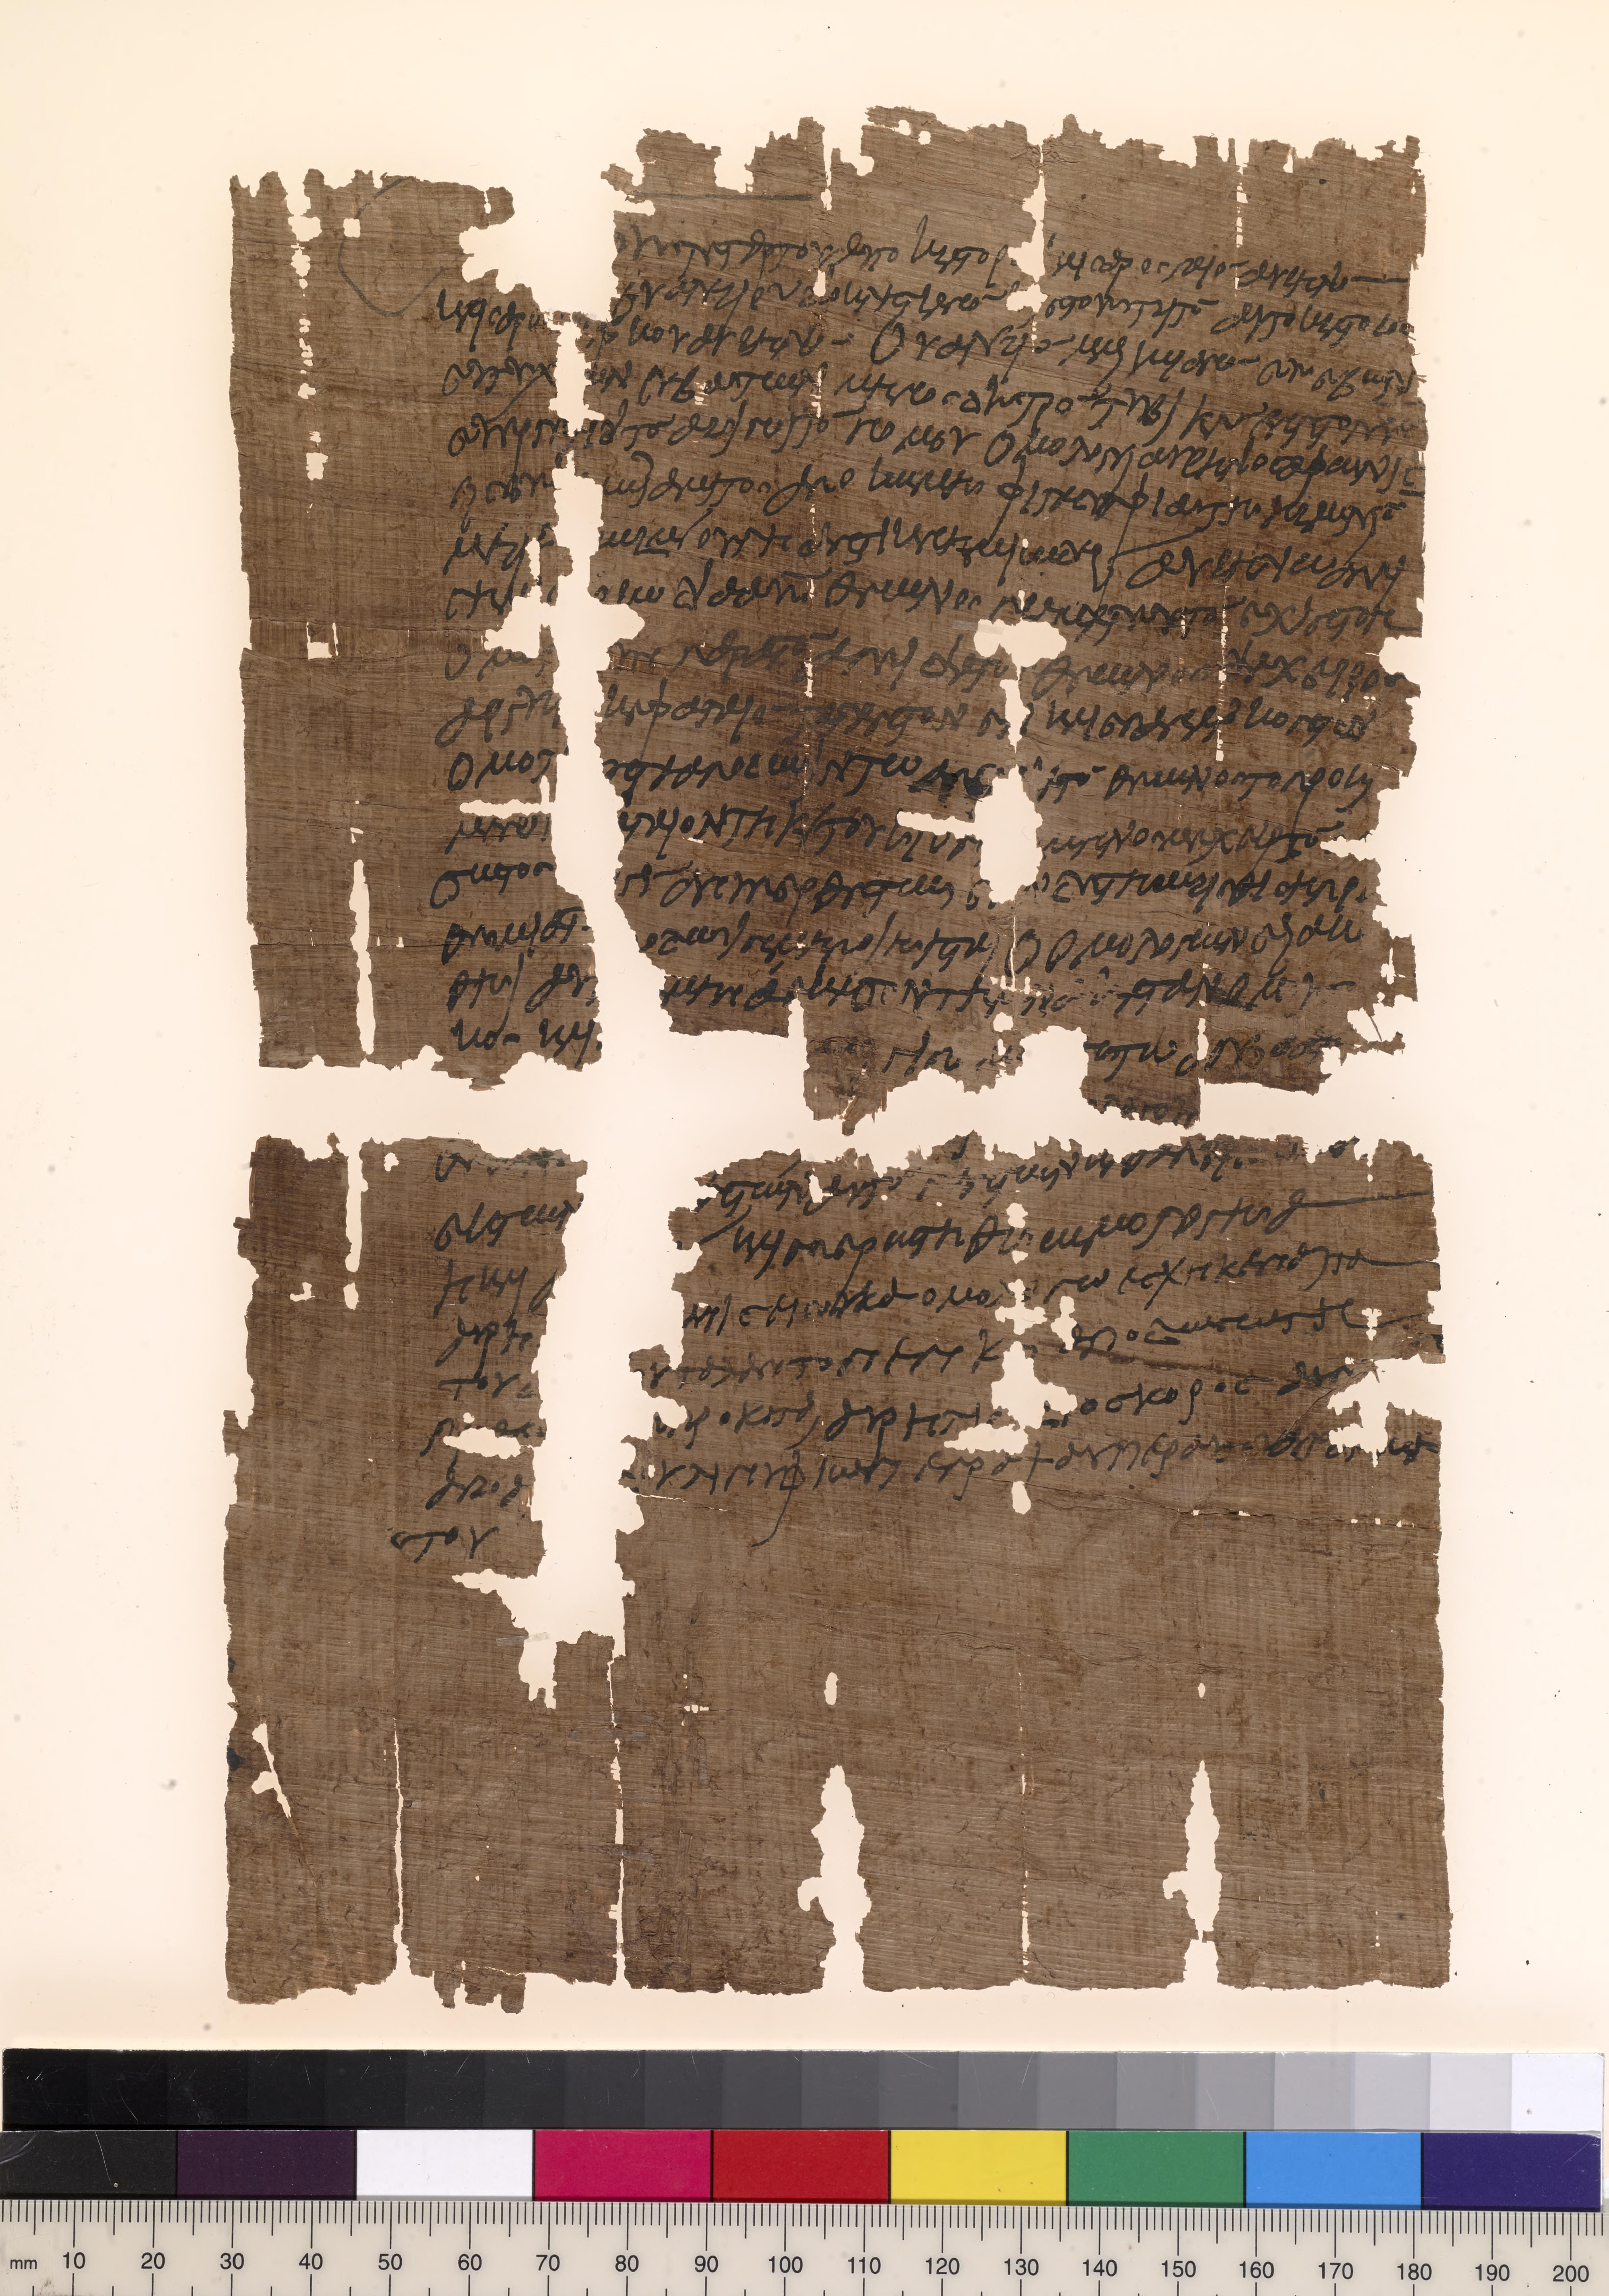
\includegraphics[width=\textwidth]{figures/0_papyri_sample.jpg}
	\caption{A papyri 1398\_1353R torn into several fragments}
	\label{fig:papyri_sample}
\end{figure}
%
\noindent Deep learning algorithms are among the commonly discussed types of algorithms when it comes to supporting papyrologists. Research has shown that the use of deep learning can increase the efficiency of papyrologists. However, even though the results are promising, there are still many unanswered questions that we do not understand. Once a better understanding of the features is obtained, the algorithms can increase the papyrologists's efficiency by a greater chance. 

\section{Contribution}
The general objective of this thesis is to make the work of papyrologists easier and increase their efficiency
by partially automating the reassembling process. To this end, an algorithm is designed to infer a
smaller sub-selection of fragments with a high likelihood of being a potential fit. In the following, this
algorithm is called puzzle-helper. Additionally algorithms have to be in a format that papyrologists can use the algorithm without a computer science background. Also, using deep learning implies that a vast amount of (labeled) data is required. The database from the University of Michigan offers plenty of it. Once the data is downloaded, it must be correctly preprocessed, like removing low contrast images or labeling the data. In particular, this thesis is centered around the following research questions:
\begin{questions}
	\item What papyrus characteristics contribute to the success of papyrus fragment retrieval?
	\item How can papyrologists use fragment retrieval model efficiently?
\end{questions}

\section{Outline}
In \Cref{chap:intro}, the context of this master thesis is explained, and the research questions are defined. Further, it is explained how the thesis is structured. \Cref{chap:Foundation} presents groundbreaking work in all areas that are relevant to this thesis. The objective is to present a quick overview of the state-of-the-art in historical fragment retrieval. \Cref{chap:Datasets} explains the creation of a dataset that can be used for papyri fragment retrieval. The objective is to guide the reader such that it is possible to recreate the dataset quickly. \Cref{chap:theory} serves as a short introduction to the field of deep learning. Further, it will be presented how that technology is used in the field of \ac{cv} for cultural heritage by the example of papyri fragment retrieval. \Cref{chap:methodology} shows how the author of this thesis used \ac{dml} as a methodology for answering the defined research questions. Further it shows how the results have been evaluated with suitable metrics. \Cref{chap:results} summarizes the results. It shows what was achieved while conducting the experiments and evaluating the results according to the defined metrics. \Cref{chap:application} shows how the results can be efficiently presented to an audience of papyrologists without \ac{cv} capabilities. \Cref{chap:discussion} revisits the research questions and summarizes the key findings. Furthermore, the results are interpreted and discussed to align with the defined research questions. Finally, the author of this thesis presents optional future work and finalizes his work with a summary.    % Einfuehrung (\chapter{Einf"uhrung})
\cleardoublepage
\chapter{Foundation}
\label{chap:Foundation}
This thesis is about \ac{dnn}, metric learning, and the retrieval of historical papyrus documents. The first part of this chapter shows chronologically why these topics matter and, more specifically, why the intersection between these topics matters. The state-of-the-art describes the former achievements and research gaps of related publications.
%
\section{History}
\label{sec:history}
As mentioned in the introduction, ancient documents are valuable as historical references. They serve as a scientific basis to confirm or reject the theories of historians, and due to the difficulty and complexity of analyzing such documents, the task is gaining interest among other scientific fields. For instance, more and more computer scientists are interested in analyzing historical documents \cite{Fiorucci20}. Several competitions were established with interests in writer identification, page retrieval, content classification, or related topics \cite{Christlein19, Cloppet17, Fiel17, Seuret20, Seuret21}. Some competitions focus on special subtasks, which are frequently used during the analysis of historical documents, for example, the separation of background and foreground \cite{Tensmeyer20}.
New datasets allow researchers to compare their methods with each others \cite{Fiorucci20, Pratikakis19}. Table \ref{tab:competitions} provides an overview of the competitions held in recent years and Table \ref{tab:datasetsOverview} shows presents an overview about available data sets. Both tables are not complete, and only presented to emphasize that the field has grown in importance in recent years.\\

\begin{table}[]
	\resizebox{\textwidth}{!}{%
		\begin{tabular}{@{}llll@{}}
			\toprule
			\textbf{Institution} & \textbf{Name}                                                       & \textbf{Year} & \textbf{Cited by} \\ \midrule
			ICDAR                & Competition on Historical Newspaper Layout Analysis (HNLA 2013)     & 2013          & 61                \\
			ICDAR                & Competition on text line detection in historical documents          & 2015          & 29                \\
			ICDAR                & Competition on Layout Analysis for Challenging Medieval Manuscripts & 2017          & 39                \\
			ICFHR & Competition on Handwritten Document Image Binarization (H-DIBCO 2018)                  & 2018 & 12 \\
			ICFHR & Competition on Document Image Analysis Tasks for Southeast Asian Palm Leaf Manuscripts & 2018 & 5  \\
			ICDAR                & Competition on Image Retrieval for Historical Handwritten Documents & 2019          & 9                 \\
			ICDAR                & Competition on Historical Book Analysis - HBA2019                   & 2019          & 3                 \\
			ICDAR & Historical Document Reading Challenge on Large Structured Chinese Family Records       & 2019 & 8  \\
			ICDAR                & Competition on Document Image Binarization (DIBCO 2019)             & 2019          & 16                \\
			ICFHR                & Competition on Image Retrieval for Historical Handwritten Fragments & 2020          & 3                 \\
			ICDAR                & Competition on Historical Map Segmentation                          & 2021          & 4                 \\
			ICDAR                & Competition on Historical Document Classification                   & 2021          & 1                 \\ \bottomrule
		\end{tabular}%
	}
	\caption{Competitions in field of computer vision and historical documents since 2013.}
	\label{tab:competitions}
\end{table}
%
\noindent As in many computer science disciplines, there is a high success rate in using \ac{dnn} in \ac{cv}, primarily when used in a multi-step process to solve complex problems \cite{jonas14}. This trend was also recognized in the field of \ac{cv} for cultural heritage \cite{Tensmeyer20}.\\

\noindent The universal approximation theorem is one reason for the success of \acp{dnn}. Mathematically speaking, any neural network architecture aims to find a mathematical function \(y = f(x)\) that can map input features \(x\) to an output \(y\). The accuracy of this function differs depending on the distribution of the dataset and the architecture of the network employed, but the function \(f(x)\) can be arbitrarily complex. The Universal Approximation Theorem states that \acp{dnn} are universal functions approximators. For every function \(f(x)\), a \acp{dnn} can find the original function \(y = f(x)\). That theorem holds for any number of inputs and outputs. Good knowledge of software engineering and powerful hardware is necessary to build and optimize deep neural networks \cite{Hornik89}.\\

\noindent That means it is theoretically possible to find these heuristics without it, but it is hard to find them in practice. Moreover, the availability of software frameworks for \acp{dnn} and powerful hardware is also part of the success. In the context of this master thesis, \acp{dnn} are theoretically capable of finding a solution for every classification or retrieval task such as finding the approximation for a function which can retrieve papyrus fragments. To obtain a well-working approximation it is necessary to implement advanced algorithms and to optimize them, utilizing powerful hardware.\\

\noindent In recent years, it has been shown that instead of learning relevant features, it is beneficial to the performance of such algorithms to learn an embedding that quantifies the similarity or dissimilarity between objects. This approach is called metric learning, and in connection with \acp{dnn}, it is called \ac{dml}.\\

Metric learning aims to reduce the distance between objects from the same category and increase the distance between objects from different categories \cite{KAYA19}. This approach has proven successful when assembling similar things like puzzles or, like in the case of this master thesis, when assembling historical documents. Deep Neural Networks that follow this approach converge faster and cope better with many different classes \cite{Lais19, Ostertag21, Pirrone21}. A more detailed introduction to \acp{dnn} and \ac{dml} is stated in \Cref{chap:theory}.\\

\noindent On the one hand, \ac{cv} for cultural heritage can benefit from \ac{dml} but on the other hand, implementing these algorithms can be tedious and time-consuming. PyTorch metric learning is an open-source library that aims to remove this barrier for both researchers and practitioners. The modular and flexible design allows users to quickly try out different combinations of algorithms in their existing code. It also comes with complete train and test workflows.\\

\begin{table}[]
	\resizebox{\textwidth}{!}{%
		\begin{tabular}{@{}lllll@{}}
			\toprule
			\textbf{Name} &
			\textbf{Description} &
			\textbf{Task} &
			\textbf{Provided at} &
			\textbf{Year} \\ \midrule
			AMADILontarSet &
			Around 26,020 images  in certain categories. &
			Text recognition &
			ICFHR &
			2016 \\
			GRK-Papyri &
			\begin{tabular}[c]{@{}l@{}}This dataset consists of 50 handwriting\\ samples in Greek on papyri.\\ Approximately from the 6th\\  century A.D., which belong to\\  10 different scribes\end{tabular} &
			Reasembling &
			ICDAR &
			2019 \\
			\begin{tabular}[c]{@{}l@{}}Sundanese\\ \\ Palm Leaf\\ Manuscript Dataset\end{tabular} &
			\begin{tabular}[c]{@{}l@{}}he dataset was constructed from \\ 66 pages of 27 collections\\ of Sundanese palm leaf \\ manuscripts from the 15th century.\end{tabular} &
			\begin{tabular}[c]{@{}l@{}}Handwriting\\ Recognition\end{tabular} &
			IAPR &
			2017 \\
			Michigan Dataset &
			\begin{tabular}[c]{@{}l@{}}1,118 papyri on 4,579 fragments\\ collected from the \\ University of Michigan\end{tabular} &
			Fragment Retrival &
			&
			2021 \\
			HisFragIR20 &
			\begin{tabular}[c]{@{}l@{}}The train set contains \\ around 100,000 fragments\\  using the HistoricalIR19 \\ as a base dataset.\\ Most of them contain\\ some text, however, some \\ fragments are quite small.\\ The test set contains about 20,000 new fragments-\end{tabular} &
			\begin{tabular}[c]{@{}l@{}}Fragment Retrical,\\ Writer Identification\end{tabular} &
			ICFHR &
			2020 \\ \bottomrule
		\end{tabular}%
	}
	\caption{Selection of public datasets.}
	\label{tab:datasetsOverview}
\end{table}
%
\noindent The challenges in \ac{cv} for cultural heritage are manifold, and the number of publications is constantly increasing. In addition, the tasks and topics are again influenced by trends within the community. For example, papyrus is becoming increasingly attractive as a material. Often neglected in the past because of its high complexity, this complexity is becoming interesting now \cite{Tensmeyer20}.\\ 

\noindent Also, when looking at the work of other computer vision practitioners, it can be noticed that other materials are analyzed first, and then the same methods are applied to papyrus documents. For example, Ostertag has shown that \ac{dml} is suitable for assembling broken clay shards \cite{Ostertag21}. In the following, Pirone first showed that this is also possible with papyrus, and then even proved that it is possible to assemble papyrus without knowing in advance to which document a papyrus fragment belongs \cite{Pirrone21}. 
%
\section{State-of-the-art}
\label{sec:stateArt}
The first authors who analyzed \ac{dml} to reassemble historical documents were Kelly Lais Wiggers, Alceu de Souza Britto Junior, Alessandro Lameiras Koerich, Laurent Heutte Luiz Eduardo Soares de Oliveira. Their publication, ``Deep Learning Approaches for Image Retrieval and Pattern Spotting in Ancient Documents'', used a \textit{Siamese Neural Network} to retrieve corresponding parts of the DocExplore dataset. A siamese \ac{nn} is a \ac{dml} architecture where weights are adjusted based on an anchor vector and a positive or negative example. That approach works well on the data compared to classical machine Learning techniques and other deep learning techniques. The publication was limited to the DocExplore dataset, and it remained open whether the approach works on a more realistic dataset \cite{Lais19}.\\

\noindent That research gap is precisely the question that Cecilia Ostertag and Marie Burton addressed in their paper ''Matching ostraca fragments using a siamese neural network'', where they answered the question if \textit{Deep Metric Learning} is suitable for matching broken clay shards. They have shown that the approach is works and a higher accuracy is possible by utilizing fine-tuned parameters and deeper networks. Furthermore, it was shown that an easy-to-use application has to be provided for historians. Otherwise, the algorithms are too complicated to be used. The question of how \textit{metric learning works} with papyrus documents were not answered \cite{Ostertag21}.\\

\begin{table}[]
	\resizebox{\textwidth}{!}{%
		\begin{tabular}{@{}llllll@{}}
			\toprule
			\textbf{Publication} &
			\textbf{Dataset} &
			\textbf{Test data} &
			\textbf{Experiment} &
			\textbf{mAP} &
			\textbf{top-1} \\ \midrule
			\begin{tabular}[c]{@{}l@{}}Deep Learning Approaches for Image Retrieval\\ and Pattern Spotting in Ancient Documents\end{tabular} &
			DocExplore &
			\begin{tabular}[c]{@{}l@{}}450 images\\ and 1464 quereis\end{tabular} &
			Image retrieval &
			0.57 &
			- \\
			Matching ostraca fragments using a siamese neural network &
			Ostraca &
			\begin{tabular}[c]{@{}l@{}}160 images\\ and 900 patches\end{tabular} &
			Image retrieval &
			- &
			0.81 \\
			Matching ostraca fragments using a siamese neural network &
			Ostraca &
			\begin{tabular}[c]{@{}l@{}}160 images\\ and 7000 patches\end{tabular} &
			Image retrieval &
			- &
			0.96 \\
			\begin{tabular}[c]{@{}l@{}}Self-supervised deep metric learning\\ for ancient papyrus fragments retrieval\end{tabular} &
			HisFrag &
			\begin{tabular}[c]{@{}l@{}}2,732 papyri on\\ 20,019  fragments\end{tabular} &
			\begin{tabular}[c]{@{}l@{}}VGG16,\\ supervised learning\end{tabular} &
			0.67 &
			0.87 \\
			\begin{tabular}[c]{@{}l@{}}Self-supervised deep metric learning\\ for ancient papyrus fragments retrieval\end{tabular} &
			Michigan &
			\begin{tabular}[c]{@{}l@{}}100 papyri on\\ 450  fragments\end{tabular} &
			Resnet50 &
			0.54 &
			0.67 \\ \bottomrule
		\end{tabular}%
	}
	\caption{Results from state-of-the-art related work.}
	\label{tab:art}
\end{table}
%
\noindent The first who addressed this question were Antoine Pirrone, Marie Beurton, and  Nicholas Journet. They analyzed the Hisfrag dataset and created a new dataset using digitalized papyri documents from the University of Michigan. More about how such a dataset can be created is presented in \Cref{chap:Datasets}. The authors used an approach similar to that of Ostertag and Wiggers. In addition, it was shown if training a model is possible even if not all information is available. More precisely, they examined what happens when a network is trained on a particular dataset and tested on another dataset of data. Additionally they experimented with self-supervised learning. That means to train a \ac{dnn} on some task A and evaluating the model on another task B. In their publication they trained a model which retrieved patches from fragments and evaluated the same model on fragment retrieval from papyrus documents \cite{Pirrone21}. All approaches worked with a \ac{map} of more than 60\%. \Cref{tab:art} summarizes the results of all three presented publications.\\

\noindent Furthermore, it was shown that the success of a deep learning architecture varies from dataset to dataset. The authors found that supervised and self-supervised learning results differ, but the difference is not proofed as statically significant. Their publication assumed that text documents more valuable for matching papyrus fragments, but that statement was not further quantified. Papyrus, unlike clay shards, has a special texture unique to each papyrus, which has not been further investigated in previous work. Therefore, the research questions listed in \Cref{chap:intro} starts exactly here and investigate the influence of these papyrus characteristics.    % (\chapter{})
\cleardoublepage
\chapter{Datasets for papyrus fragment retrieval}
\label{chap:Datasets}
%Short Intro what I do here

The following chapter describes how the raw data was processed to obtain different training, validation, and test subsets. First, it is clarified where the raw data comes from and why this reference was chosen. Then the individual processing steps are explained. 

\section{Collecting raw papyri data}
All data used in this thesis comes from the Advanced Papyrological Information System (APIS), provided hosted by the University of Michigan. APIS is a digitized version of the university's papyrus collection. Users can retrieve high-resolution digital images and detailed catalog records on papyrus characteristics, corrections to published papyri, and republications.
The information system and the resulting datasets were used several times in the field of \ac{cv} for cultural heritage \cite{Pirrone21, Ostertag21}. The information systems papyri-data is also used in the following thesis to compute comparable results. A simple but efficient bash script was used to retrieve the raw data.
 

\section{Analyzing raw papyri data}
After running the script, 8,857 papyrus documents (11.3 GB) are available. \Cref{fig:papyri_sample} shows an example of the downloaded images. As shown in the example, 96\% of the raw image data has a ruler and a color scale. That is useful for resembling papyri fragments manually. These tools are also used in computer vision, for instance, to calculate the original size of the images. That is useful because the image size often varies significantly. For example, the height of the images ranges from 789 pixels to 22,952 pixels and the width from 873 to 18,440 pixels. In \Cref{fig:distribution_image_size}, it can be seen that on the one hand, the maximum pixel values are outliers. On the other hand, it can be seen that the variance is significantly higher in comparison to standardized equally sized datasets like the cifar1000. Cifar1000 is a benchmark dataset that is oftentimes used to train machine learning and \ac{cv} algorithms and it is widely used. Since the vast difference in size was approached differently during the work for that thesis, the information given by the ruler was not used. The details of that approach are described in \Cref{sec:fragmentation}. 

\begin{figure}[t]
	\includegraphics[width=\textwidth]{figures/1_distribution_size.png}
	\caption{Distribution of image sizes (pixels) along the vertical and horizontal axis within the raw image data.}
	\label{fig:distribution_image_size}
\end{figure}

\section{Decomposition of raw papyri data into natural fragments}
\label{sec:deseperation}
In order to obtain a realistic evaluation, the final subsets should contain as many natural fragments as possible. In the raw dataset, 63\% of all images include multiple papyri fragments. Thus, the first objective of the preprocessing is to separate the raw data such that each image only shows a single papyri fragment. Furthermore, the ruler and the color scale are no longer helpful for creating predictions. In conclusion, they must be removed. Figure \ref{fig:papyri_preprocessing} shows the process from a raw papyri image towards the separated natural fragments. The main idea is to binarize the image with a histogram. White pixels correspond to the papyri fragment, and black pixels are the background. Then, bounding boxes are used to label the region around each fragment such that it is possible to separate them.\\

\begin{figure}[t]
	\includegraphics[width=\textwidth]{figures/2_papyri_preprocessing.pdf}
	\caption{Preprocessing pipeline examined on the image \text{12830\_4433LR}.}
	\label{fig:papyri_preprocessing}
\end{figure}

\noindent Noise in the images decrease the binarization quality and therefore makes it harder to find a good-fitting bounding box. A \textit{Gaussian Filter} with a blurry factor of $\sigma=95$ reduced the image noise and makes the algorithms more stable. At the same time sticking out fibers are not blurred out. After the image has been denoised, a histogram is used to find a suitable binarization decision boundary. For papyri data, it seemed reasonable to choose 86\% intensity as a threshold. That means pixels higher than 86\% intensity will be classified as background, whereas pixels with a lower intensity will be recognized as papyri. In the upper right part of Figure \ref{fig:papyri_preprocessing}, the images still contain the color scale and the ruler, which are usually identified as a papyri fragment. These two interfering objects must be removed before suitable bounding boxes can be found. An algorithm slices the image around these edges where so-called objects were found. An object is defined as a contiguous pixel set with specified size (buffer). The pixels of an object must belong together but have no connection to other objects in the image, such that natural fragments will not be removed. In the next step, convex hulls are calculated. The convex hull of a set of pixels is defined as the smallest convex polygon encloses all of the points in the set. Additionally, a mask is needed because the hull is just a line-shaped boundary that encloses the corresponding pixels. The following approach was applied on each image to create the convex hull masks: 

\begin{enumerate}
	\item Compute the x- and y-coordinates for all points along the center of each edge of each foreground pixel.
	\item Use the quickhull-algorithm to compute the convex hull of the identified points from step 1. 
	\item Use the convex hull computed in step 2 to convert the convex hull to a binary image mask.
\end{enumerate}

\noindent The name of the quickhull algorithm comes from quicksort, which was the inspiration for the developers as they designed it \cite{Barber96}. Quickhall and quicksort share the divide and conquer algorithm design paradigm. That means the algorithms recursively subdivide the problem into sub-problems until these become simple enough to be solved. Since the principle ensures efficient algorithms, it is used for many computer science-related problems such as sorting (quicksort-algorithm), computing the discrete Fourier transform (FFT-algorithm), or in the case of the thesis computing the convex hull (quickhull-algorithm). The algorithm will process as follows to find the convex hull of the papyri fragments: 
\begin{enumerate}
	\item The points on the outer ages of the x-dimension got identified. These points form a line to divide the two pixels into two subsets. The recursion will then process each subset individually.
	\item A point is identified with the highest distance to the line. That particular point forms a triangle between the point itself and the points who are on that line. The points enclosed by the triangle are not part of the convex hull - therefore, they are no longer used in the next recursing steps. 
	\item As long as points are left, the recursion will be repeated for both new sides of the triangle. 
\end{enumerate}

\noindent Figure \ref{fig:convex_hull} visualizes the procedure of finding bounding boxes. In the penultimate step, all objects are classified individually. It is essential to define the minimum size of the objects because, in the previous step, convex hulls may have been formed around tiny objects. Finally, each labeled object is stored as a single fragment. The objects are filled with a white background to obtain a rectangular or square shape. How the data looks after the preprocessing steps were applied onto the raw data, can be seen in Figure \ref{fig:sample_grid}.

\begin{figure}[t]
	\label{fig:convex_hull}
	\includegraphics[width=\textwidth]{figures/3_convex_hull.pdf}
	\caption{The convex hull algorithm for finding the bounding boxes.}
\end{figure}


\section{Computing train, test and validation subsets}
\label{sec:trainTestSplit}

It is considered best practice to divide the available data into different subsets for training, testing, and evaluating generated models. Even this best practice has some weaknesses, it is still considered the gold standard in machine learning \cite{Tan21}. It is also vital not to use the test data until the modeling is finished. The evaluation of data science projects refers to the results that the best model combined with the unseen data has achieved. Since, in real-world applications, data is also unseen, that practice ensures higher reliability. However, that procedure was done twice this master thesis due to an implementation error. Since the first iteration results are not evaluated or discussed anymore, the best-practice-paradigm is still fulfilled.\\

\noindent The distribution must be as close to the original as possible to split the data right. Additionally, the distribution must be close to a related domain-specific dataset. Otherwise, a comparison is difficult since improvements are caused by different distributions instead of more sophisticated methods. The Michigan Dataset mentioned in \Cref{sec:stateArt}) is used as a reference dataset within the following thesis. On average, it has four fragments per papyri. The dataset created during the thesis has similar values. Precisely the training set has 3.51, the validation set has 3.45, and the test subset 7.52 fragments per papyri. Both the Michigan and FAU test datasets consist of 100 papyri, but the number of papyri in the validation and training datasets are different.\\ 

\begin{figure}[t]
	\includegraphics[width=\textwidth]{figures/4_distribution_datasets.png}
	\caption{Distribution of the number of fragments per papyri on the train, test and unused subsets.}
	\label{fig:HistogramTrainTestValSplit}
\end{figure}

\noindent The Michigan dataset contains 1,000 papyri to train models and 100 papyri to validate models. In contrast, the FAU dataset consists of  422 papyri for training and 422 papyri for validation. Thus, models in the following thesis are trained on fewer examples but tested on more examples. The software architecture which has been implemented did not allow different numbers of papyri during training and validation. Moreover, it was easier to evaluate the model's performance if the number of papyri is identical, at least in the training and validation phase. \\

\noindent After all natural fragments have been separated into unique images, the distribution of that data had two noticeable characteristics. First, there are positive and negative outliers in the number of fragments per papyrus. Second, many papyri are not fragmented. The FAU dataset shall represent a real-world dataset. So, there are no artificially created fragments in any of the datasets. Instead, classes with only one fragment per papyrus, and classes with more than 60 fragments per papyri are removed. The result is a somewhat smoothed distribution. The following algorithm was applied to create a subset for training, validation, and testing:

\begin{enumerate}
	\item Order the classes according to the number of fragments of papyri. 
	\item Alternately add a class to the test, training, or validation subset until there are 100 classes in the test subset. 
	\item Repeat the procedure with the remaining classes only on the training and validation subset.
\end{enumerate}


\noindent Figure \ref{fig:HistogramTrainTestValSplit} visualizes the distributions of the individual subsets and compares them to the unused data. Additionally, three .csv files were computed to preprocess the data further.

\section{Data augmentation of papyri data}
\label{sec:fragmentation}
As described in the raw data section, the available raw data vary considerably in height and width. In addition, several images are extensively large. That makes the use of \acp{dnn} difficult. However, much of the information contained in the image is repetitive. It has already been shown that training on whole images is can be avoided. Instead, it can be sufficient to identify small representative patches of an image and train the predictive model on them \cite{Pirrone21, Ostertag21}. In this thesis, these representative patches are extracted as follows:
%
\begin{enumerate}
	\item Divide the image into \(m \times m\) non-overlapping patches.
	\item Compare all detected parts with a metric.
	\item Select the \(n\) best parts according to the selected metric.
\end{enumerate}
%
The selected metric can be used to focus on different image parts. For example, the variance as a metric ensures that mainly the outer edges of a fragment are selected (Figure \ref{fig:patchSelection}). Before the patches are evaluated, it will be ensured that there is enough papyri surface on each patch. Therefore the intensity mean of each channel gets calculated. If the sum of these means is lower than 80\%, the patch will not be used. One exception is the first metric (random). Here the random choice was made between all patches. If there are not enough patches to fulfill these property, the patches with the most papyri surface get selected even there are almost white. That can slow down the performance but to form comparable batches it was decided not to use a different number of patches per fragment. That topic will be discussed in greater detail in chapter 5. 
%
\begin{figure}[t]
	\label{fig:patchSelection}
	\includegraphics[width=\textwidth]{figures/5_patch_selection_algortihm.pdf}
	\caption{A metric changes the way how patches got selected.}
\end{figure}
%
\begin{table}[]
	\centering
	\resizebox{\textwidth}{!}{%
		\begin{tabular}{lllll}
			\hline
			\textbf{\#} & \textbf{name} & \textbf{selection procedures} & \textbf{patch\_size} & \textbf{n} \\ \hline
			0 & baseline\_small\_small & random & 64 & 5 \\
			1 & baseline\_small\_big & random & 64 & 20 \\
			2 & baseline\_medium\_small & random & 128 & 5 \\
			3 & baseline\_medium\_big & random & 128 & 20 \\
			4 & baseline\_big\_small & random & 256 & 5 \\
			5 & baseline\_big\_big & random & 256 & 20 \\
			6 & mean\_small\_small & intensity-mean & 64 & 5 \\
			7 & mean\_small\_big & intensity-mean & 64 & 20 \\
			8 & mean\_medium\_small & intensity-mean & 128 & 5 \\
			9 & mean\_medium\_big & intensity-mean & 128 & 20 \\
			10 & mean\_big\_small & intensity-mean & 256 & 5 \\
			11 & mean\_big\_big & intensity-mean & 256 & 20 \\
			12 & text\_small\_small & prefer text & 64 & 5 \\
			13 & text\_small\_big & prefer text & 64 & 20 \\
			14 & text\_medium\_small & prefer text & 128 & 5 \\
			15 & text\_medium\_big & prefer text & 128 & 20 \\
			16 & text\_big\_small & prefer text & 256 & 5 \\
			17 & text\_big\_big & prefer text & 256 & 20 \\
			18 & h\_text\_small\_small & highlight text & 64 & 5 \\
			19 & h\_text\_small\_big & highlight text & 64 & 20 \\
			20 & h\_text\_medium\_small & highlight text & 128 & 5 \\
			21 & h\_text\_medium\_big & highlight text & 128 & 20 \\
			22 & h\_text\_big\_small & highlight text & 256 & 5 \\
			23 & h\_text\_big\_big & highlight text & 256 & 20 \\
			24 & h\_fibers\_small\_small & highlight background & 64 & 5 \\
			25 & h\_fibers\_small\_big & highlight background & 64 & 20 \\
			26 & h\_fibers\_medium\_small & highlight background & 128 & 5 \\
			27 & h\_fibers\_medium\_big & highlight  background & 128 & 20 \\
			28 & h\_fibers\_big\_small & highlight background & 256 & 5 \\
			29 & h\_fibers\_big\_big & highlight  background & 256 & 20 \\ \hline
		\end{tabular}%
	}
	\caption{Overview of the created datasets.}
	\label{tab:datasets}
\end{table}

\begin{figure}[t]
	\label{fig:dataset}
	\includegraphics[width=\textwidth]{figures/6_datasets.pdf}
	\caption{The papyri patch representations from dataset 1 to 5.}
\end{figure}

\subsection{Random}
The metric "random" means that patches get selected randomly among each computed patch. The resulting datasets are created to obtain baseline results. Suppose there is no significant increase in the model performance compared to that dataset, then it is useless to apply a metric at all, especially since applying a metric is computationally expensive. Figure \ref{chap:Datasets} shows a papyrus image and its representations by random patches with different \(m\) and \(n\) values (dataset 0 - 5).

\subsection{Mean}

That metric chooses the patches where the patch intensity-mean is close to intensity mean of all fragments. It will be processed as follows to obtain suitable patches according to that metric:
\begin{enumerate}
	\item Calculate the pixel mean of each patch channel.
	\item Calculate the absolute difference between the calculated patch channel mean and the global channel means.
	\item Select the patches where the sum of the differences calculated in step 2 is the lowest. 
\end{enumerate}

\begin{figure}[t]	
	\includegraphics[width=\textwidth]{figures/7_dataset_2.pdf}
	\caption{The papyri patch representations from dataset 6 - 11.}
	\label{fig:dataset2}
\end{figure}

The global channel intensity-mean values have been calculated before. The fragments were binarized (\ref{sec:deseperation}), and then the average channel mean of 100 fragments was evaluated. Since the mean will be shifted towards background areas, binarization was necessary to obtain more accurate results. That metric was chosen to select images close to the original image regarding their color distribution. Thus were are a representative subset of all pixels of the unpatched papyri image. Figure \ref{fig:dataset2} shows a papyrus image and representative patches with different \(m\) and \(n\) values (dataset 6 - 11).


\begin{figure}[t]
	\includegraphics[width=\textwidth]{figures/8_dataset_3.pdf}
	\caption{The papyri patch representations from dataset 12 - 17.}
	\label{fig:dataset3}
\end{figure}

\subsection{Prefer Text}
Prefer text means that the patches with the highest text pixels are selected. A simple heuristic is used to determine the number of text pixels. After visual confirmation, that heuristic seems as reliable as more complicated computations. For the heuristic, each gray-scaled patch is locally thresholded with a threshold of 2\% intensity. Afterward, the remaining foreground pixels get counted and used as a score. In images with different intensities and color distribution, that score selected the patches with the most text onto them. If there are no text pixels on the patches, the patches with the most papyri pixels get selected. Figure \ref{fig:dataset3} shows a papyrus image and the selected text patches with different m and n values (dataset 0 - 5).


\subsection{Highlight metrics}
Highlighting text and fibers are more advanced metrics, and their calculation uses state-of-the-art binarization and inpainting. That task is regarded as the thesis's second milestone and will be described in Chapter 2. 

\begin{figure}[t]
	\includegraphics[width=\textwidth]{figures/9_sample_grid.pdf}
	\caption{Natural papyri fragments after applying the raw data decomposition.}
	\label{fig:sample_grid}
\end{figure}





   % (\chapter{})
\cleardoublepage
\chapter{Theory}
\label{chap:theory}
\Cref{chap:theory} describes the necessary theory to understand how \ac{dml} is used to retrieve papyrus fragments. Therefore, the fundamentals of \acp{ann} are presented in \Cref{sec:anns} and the fundamentals of \acp{cnn} are explained in \Cref{sec:cnns}. The material for the introduction is used from the lecture Deep Learning, hosted by the department for Pattern Recognition at the University of Erlangen-Nuremberg\footnote{The complete ''Deep Learning'' lecture is available on  \href{https://www.youtube.com/watch?v=p-_Stl0t3kU&list=PLpOGQvPCDQzvgpD3S0vTy7bJe2pf_yJFj}{YouTube} and the \textit{Data Science} blog \href{https://towardsdatascience.com/all-you-want-to-know-about-deep-learning-8d68dcffc258}{Towards Data Science}.}.   

\section{Artificial neural networks}
\label{sec:anns}
\acp{ann} are computational models, consisting of multiple neuron layers, inspired by the human brain. The neurophysiologist Warren Sturgis McCulloch and the logician Walter Pits first mentioned that type of model. In their publication ''A logical calculus of the ideas immanent in nervous activity'', the scientists define a logical model inspired by the brain, for calculating complex decisions \cite{mcculloch43a}. Frank Rosenblatt took up this idea and invented the perceptron. Today, this model is the conceptual foundation for all kinds of \acp{ann} \cite{rosenblatt1958perceptron}.\\

\subsection{Perceptron}
\label{subsec:perceptron}
\begin{figure}[t]
	\includegraphics[width=\textwidth]{figures/10_perceptron.pdf}
	\caption{Computation graph of a perceptron.}
	\label{fig:perceptron}
\end{figure}
%
\noindent The perceptron is a mathematical function that assigns a binary value \(\hat{y}\) to an input vector \(x\).
The computation graph in \Cref{fig:perceptron} visualizes the Perceptrons functionality. As shown in the weights part of the figure, each input value \(x_i ... x_n\) will be multiplied with an adjustable weighting term \(w_i ... w_n\). Afterwards and as depict in the sum part the \(z\)-values are summarized by taking the product of \(z_i ... z_n\). As described in the threshold part of \Cref{fig:perceptron}, the result is evaluated on a threshold. Finally the output part explains that if the resulting sum exceeds the threshold, the function returns one, otherwise, it returns zero.\\

\noindent While training, the algorithm adjusts \(w\) to compute the desired output. Since the ability of learning suitable weights is some form of learning, the perceptron is regarded as a simple form of artificial intelligence. Given multiple input vectors \(x\) (inputs) and corresponding output values \(y\) (samples), the objective of a trained perceptron is that it returns \(\hat{y} = y\). Instead of explicit programming, the weights are randomly initialized and then iteratively adjusted as long as the algorithm converges. Convergence means, the difference \(\hat{y} - y\) (loss) does not change significantly anymore because it has reached a local optimum. For instance, if the input is a value \(x \in \mathbb{Z}\) the perceptron return \(1\) if \(x > 0\). In the training procedure the learns to approximate the underlying function, by increasing the weights if  \(x \cdot w - b < 0 \) or decreasing the weights if \(x \cdot w - b > 0 \). The mathematical definition of this function is given by the following expression, where the subscript \(i\) stands for an entity in \(x\):
%
\begin{equation}
	\hat{y} = \left\{\begin{array}{lr}
		1 & \text{for } \sum x_i w_i > threshold\\
		0 & \text{for } \sum x_i w_i \le threshold\\
	\end{array}\right\}
\end{equation}
%
\noindent The given expression can not be directly implemented. The expression can be simplified by replacing the sum terms with a dot product and introducing a bias term \(b= - threshold\): 
%
\begin{equation}
	\hat{y} = \left\{\begin{array}{lr}
		1 & \text{for } w \cdot x - b > 0\\
		0 & \text{otherwise}\\
	\end{array}\right\}
\end{equation}
%
\noindent On one hand, the perceptron finds correct weights to obtain the logical operations AND, OR, and NOT. On the other hand, the perceptron can only determine heuristics for functions in which the output is linearly separable. That is not the case for the logical XOR function. Thus, a perceptron can not find correct weights such that the output is identical to the XOR function (XOR-problem). If a smoother function (activation function) is applied to the weighted sum of \(x \cdot w\), data must no longer be linearly separable. Thus, the XOR problem is solvable. This generalized form of the perceptron is called unit or neuron. An example of an activation function is the \ac{relu} or the sigmoid function. The sigmoid function can scale the output values between 0 and 1. That makes the function interpretable as an output probability for classification tasks. Furthermore, an activation function ensures that the neuron is differentiable. Without differentiable neurons, training algorithms such as gradient descent do not work.  
%
\subsection{Deep neural networks}
\Cref{fig:MLP} shows a so-called multi-layer perceptron or \ac{nn}. That type of network consists of an input-layer (left-hand side), multiple hidden-layer (middle part), and an output-layer (right-hand side). The input-layer does not perform any calculation, whereas the hidden layers and the output layer combine multiple neurons. If more than three hidden-layers are used, the network is considered as a \ac{dnn}. The number of input neurons is equal to the size of the input vector, and the number of neurons in the output layer corresponds to the performed task. For instance, if the \ac{dnn} is used to classify papyri fragments, then the number of input neurons is equal to the number of pixels times 3 (each for one color channel). The number of output neurons is equal to the number of distinct types of papyri (classes).\\

\begin{figure}[t]
	\includegraphics[width=\textwidth]{figures/11_multi_layer_perceptron.pdf}
	\caption{Architecture of a fully connected \ac{dnn}.}
	\label{fig:MLP}
\end{figure}
%
\noindent As visualized in \Cref{fig:MLP}, each neuron is connected to any other neuron (fully connected). That property allows the fully connected \ac{nn} to approximate arbitrary function and hence to become universal function approximator. These networks can not be trained in the same manner as a perceptron. Instead, the backpropagation algorithm is used to obtain suitable weights iteratively \cite{Rumelhart86}. The algorithm propagates the loss backwards through the \ac{dnn} to obtain gradients of the loss function. The gradient of a function is its change rate, pointing in the direction of the steepest ascent. For the calculation of gradients, a differentiable activation function is obligatory. Thus, the optimization via the backpropagation algorithm will not work (\Cref{subsec:perceptron}).
%
\subsection{Terminology}
Domain-specific terminology is often used to describe the characteristics of a \ac{dnn} (architecture) and to discuss their results. The following list will enable the reader to understand the explanations and discussions regarding \acp{dnn} used within this thesis:
%
\begin{enumerate}
	\item The term \textbf{architecture} refers to the number of neurons and layers which is used during the training. Furthermore, the architecture describes the types of neurons and layers used. As described in \Cref{sec:cnns}, fully connected \ac{nn} are just one type of \acp{dnn}. In recent years many distinct architectures have been introduced. The architectures are usually highly specialized for a specific field such as \ac{cv} tasks. For instance the ResNet19 or the DenseNet121 architectures. These architectures are also used within this thesis and described in \Cref{subsec:drl} and \Cref{subsec:dcn}.
	\item The \textbf{cost function} and the \textbf{loss function} are functions to determine the performance of a \ac{dnn}. For instance, the binary triplet loss (\Cref{sec:dml}). The terms cost function and loss function almost refer to the same meaning. A loss function mainly applies for a single training sample whereas the cost function is the average of multiple loss functions, evaluated on batches of outputs.
	\item The \textbf{optimizer} is an optimization algorithm that iteratively minimizes the cost function by adjusting the weights. There are many different optimizers, but almost all algorithms share the fundamental principle of gradient descent.
	\item \textit{Overfitting} means that a \ac{dnn} rather absorbs and stores the information presented as it was shown via examples instead of learning domain-specific characteristics (features) such that the model performs well on unseen data. 
\end{enumerate}
%
\section{Convolutional neural networks}
\label{sec:cnns}
\acp{cnn} are also inspired by biology and mimic the visual cortex, in which neurons act as receptive fields, and turn active when specific patterns appear. For instance, some neurons turn active if an edge appears, and other neurons are more sensitive to complex patterns such as the human eye. Neurologists agree that the fundamental principle of how the brain works is still unknown \cite{Savage19}. Thus, \acp{cnn} and \acp{dnn} are not accurate models of the biological brain.\\

\begin{figure}
	\label{fig:convs}
	\includegraphics[width=\textwidth]{figures/12_convolution_operation.pdf}
	\caption{Convolution explained in three layers of abstraction.}
\end{figure}
%
\noindent However, in 1989, LeCun et al. applied a \ac{cnn} to the task of handwritten digit recognition \cite{lecun-90c} and achieved outstanding results. As a result, \acp{cnn} gained on popularity. Finally, Kizhevsky et al. have presented a \ac{cnn} which outperformed any other model on the \ac{imagenet} dataset. That dataset was published along with a challenge and is used to create benchmarks for object classification tasks. The \ac{imagenet} dataset consists of hundreds of object categories and millions of images \cite{ILSVRC15}. Since AlexNet won the challenge, \acp{cnn} become the state-of-the-art architecture in the field of \ac{cv} \cite{Schmidhuber15}. In their publication, Kizhevsky and his colleagues predicted that if \ac{gpu} power is increasing, future architectures will achieve outstanding results in many distinct \ac{cv} domains \cite{NIPS2012_c399862d}.\\

\noindent The fundamental component of a \ac{cnn} is the convolution layer. It slides a kernel (filter) multiple times across the input to detect specific features. \Cref{fig:convs} visualizes the convolution operation on three levels of abstraction. In the bottom row, the convolution is presented in form of linear algebra. Linear algebra provides the first steps into vectorization, presenting a deeper way of thinking about parallelization. Machine learning models such as linear regression use these techniques to determine heuristics in a sufficient time. In the middle part of \Cref{fig:convs}, the inputs and outputs of such operations are visualized. On the left-hand side, a fragment is separated into squares to visualize that the algorithm summarizes the information from these squares. It is not necessarily the case that the filter is applied on non-overlapping squares. Instead, it can be moved across the image in every arbitrary format. The middle part of the figure shows a filter which summarizes the information given by each square. The right hand side of the image depicts the result. It only shows the edges of the original image. Thus it the filter, removes each feature which does not contain information about edges. That result is called a feature map, since it maps the important features from an input tensor onto an output tensor. In the first row, the mathematical symbol representations are presented. Given the mathematical symbol representation, a convolution is mathematically defined as follows:
\begin{equation}
	(f \ast g) (x) = \int_{-\infty}^{\infty} f(\tau)g(x-\tau)d\tau
\end{equation}
\noindent where
\begin{itemize}
	\item \(f \ast g\) means to convolve (\(\ast\)) a kernel \(f\) with an input signal \(g\) at position \(x\)
	\item \(-\tau\) means flipping the signal,
	\item \(x\) stands for moving to the desired position , 
	\item and \(\int_{-\infty}^{\infty}\) stands for accumulating every interaction 
\end{itemize}
\noindent Each filter has adjustable weights and performs a convolution operation to make specific features visible in the feature maps. Therefore, the training of a \ac{cnn} works as follows:
\begin{itemize}
	\item A \ac{cnn} adjusts weights of small filters such that they become feature detectors.
	\item These feature detectors are applied across the input such that it scans small patches of the input for these features. 
	\item This operation is subsequently applied multiple times such that the network learns to detect low-level features (e.g., edges) in the first layers and features of features (e.g., a letter on a papyri image) in deeper hidden layers.
	\item Pooling is used to summarize the information stored in the filters and decrease the network's size. Pooling works again by sliding a filter across the feature maps. In contrast to the filters in the convolution layers, these filters do not have adjustable weights. There are different variations of pooling, such as max-pooling or average pooling. For example, max-pooling uses filters to retain the maximum value of an area. 
\end{itemize}
The authors of the first \acp{cnn} already assumed that not every layer is useful in some tasks. Hence, it is more efficient to skip layers instead of optimizing them. That assumption leads to deep residual networks. 
%
\subsection{Deep residual learning}
\label{subsec:drl}
\begin{figure}[t]
	\centering
	\includegraphics[width=100mm]{figures/13_residual_improve_performance.png}
	\caption{Training error (left) and test error (right) on CIFAR10 with 20 layers and 56 layer plain networks \cite{He15}.}
	\label{fig:modelperformance}
\end{figure}
%
\noindent Adding more layers (filters) leads to an increase in performance, but at some point, the improvement saturates. Kaiming et al. proved that overfitting does not cause this saturation because the performance also saturates in the training procedure. Hence, the full potential of deeper networks is not completely used \cite{He15}. \Cref{fig:modelperformance} shows an example of a 20 layer network with a lower training and test error as the architecture with 56 layers. To solve a more complex problem, researchers applied more and more layers in. The intuition behind their approach is that these layers progressively learn more complex functions. This problem of training very deep \acp{dnn} has been alleviated with the introduction of the ResNet architecture, short for Residual Networks. It is a specific type of \acp{dnn} that was introduced in 2015 by Kaiming He et al. in their paper ''Deep Residual Learning for Image Recognition'' \cite{He15}. ResNets consist of residual blocks, as presented in \Cref{fig:residual}. Compared to earlier \ac{cnn} architectures, there is a direct connection that skips some layers in between. This connection is called skip connection and it solves the vanishing gradients in \acp{dnn} because the skip connection allows the gradient to flow through. In a \ac{dnn}, the vanishing gradient problem is encountered when training \acp{ann} with gradient-based the backpropagation algorithm. During each iteration of training each of the \ac{nn}'s weights receives an update proportional to the partial derivative of the error function with respect to the current weight. Sometimes the gradient will be vanishingly small. Thus the update and therefore the learning effect is vanishingly small as well. This can completely stop the \ac{nn} from further training. Skip connections allow to learn identity functions, ensuring that the higher layer will perform at least as good as the lower layer. For instance, a \ac{dnn} with \(n\) layers, in which the output of a layer \(y_n\) is given by the function \(y_n = H(y_n - 1)\). In that case, a skip connection's mathematical definition means adding the identity function to enable the network to bypass one or multiple layers. If the identity path skips only one layer, the mathematical definition is as follows:
\begin{equation}
	x_l = H(x_{l-1}) + x_{n-1} \approx F(x_{l-1})
	\label{equ:skip}
\end{equation}
where 
\begin{equation}
	H(y_{n -1}) \approx F(x_{n-1}) - x_{l-1}
\end{equation}
\noindent Adding skip connections does not increase the number of parameters and does not increase the computational complexity of a \ac{dnn} architecture. He et al. showed that \acp{dnn} benefit from the skip connections and argued that this is due to the better preconditioning of the optimization problem. The authors proved that the residual functions of a \ac{dnn} are not as activated as functions in other \acp{dnn} architectures. They stated that the loss function of the weight layers are closer to the identity function in comparison to a zero-mapping. He et al. concluded that this observation causes the improved optimization behavior. So to speak, in a deep residual network, it is safe to train very deep layers in order to get enough learning power. In the case of a degenerated performance, layers can learn to be an identity function and do no harm to performance.
%
\begin{figure}[t]
	\centering
	\includegraphics[width=50mm]{figures/14_residual_block.png}
	\caption{The skip connections as main building block of residual learning \cite{He15}.}
	\label{fig:residual}
\end{figure} 
%
\subsection{Densely connected networks}
\label{subsec:dcn}
Densely connected networks further exploit the application of skip connections. Inspired by ResNets, Huang Gao et al. invented a network architecture where each layer has a skip connection to every other layer \cite{Huang17}. In ResNets, the identity function and the output of certain layers are combined by the summation of the output and the identity function. Gao et al. changed that behavior such that the input of the subsequent layer includes the input of the preceding layers. Each layer has access to the feature maps of all preceding layers. A concatenation term is used instead of the summation as presented in \Cref{equ:skip}. That changes the expression as follows:
\begin{equation}
	\label{equ:skip2}
	x_l = H([x_{0},x_{1},...,x_{l-1}]) \approx F(x_{l-1})
\end{equation}
So to speak, instead of only learning an identity mapping, the algorithm has a direct connection to every result achieved in higher layers. \Cref{fig:dense} visualizes the architecture of a densely connected network. The authors cite that their architecture beats the results of the other competing architectures, such as ResNet in experiments on the \ac{imagenet} challenge. That statement will be evaluated on the the papyri datasets which have been introduced along this thesis in  \Cref{sec:Experiments}. 

\section{Deep metric learning}
\label{sec:dml}
\begin{figure}[t]
	\centering
	\includegraphics[width=\textwidth]{figures/15_metric_learning_dark_mode.pdf}
	\caption{\textit{Metric Learning} for papyri fragment retrieval.}
	\label{fig:FigureML}
\end{figure} 
%
\ac{dml} is a technique to quantify similarities and dissimilarities between classes. For instance, it determines the equality of two papyrus fragments by an output value, expressed by a distance metric. Considering the topic of this thesis, the algorithm embeds the papyrus fragments into another dimension, such that the embeddings become separable. Precisely, embeddings from the same papyrus document shall appear rather close to each other and vise versa, embeddings from distinct papyri shall appear wide apart.\\

\noindent That desired behavior of an metric learning algorithm is visualized in \Cref{fig:FigureML}. On the left-hand side, two distinct papyri consist of two fragments. The center of \Cref{fig:FigureML} is a visualization of four embeddings created by an untrained \ac{dml}. The green embeddings in light and dark green represent Papyri A, and the light and dark brown embeddings represent Papyri B. If the model is not trained, the embeddings mostly do not group at all. After training, the green and brown embeddings will group, and the total distance between green and brown values increases, as can be seen on the right-hand side of \Cref{fig:FigureML}. \\

\noindent Recently, \ac{dl} has proven to be an effective end-to-end approach for building metric learning algorithms. End-to-end in this context means that the transformation from the input feature space to a useful embedding space and the discrimination of that space is realized through one process. If \ac{dl} and metric learning are applied together, researchers use the term \ac{dml}. A loss function is applied such that the model serves as a feature extractor and feature discriminator at the same time. By using that approach, researchers achieved competitive results in certain research fields such as facial recognition and image classification \cite{Duan18, Dai18, Kim_2018_ECCV}. Moreover, \ac{dml} was successfully applied to the task of papyrus fragment retrieval (\Cref{chap:Foundation}, \Cref{sec:stateArt}).\\

\noindent In comparison to traditional \ac{dl} techniques such as \acp{cnn}, \ac{dml} has a stronger ability to cover input characteristics. That is one of the reasons why \ac{dml} is thriving on tasks in which it is important to distinguish between small characteristics. Another strength of \ac{dml} is its ability to compute robust classifiers if the number of classes is high \cite{Schroff15, Rippel16}. 

\subsection{Triplet loss function}
\label{subsec:tripletloss}
Triplet loss is used to guide the optimizer such that the distance between negative and anchor embeddings increases and the distance between anchor embeddings and positive embeddings decreases \cite{Schroff15}. Mathematically this can be expressed as follows: 
\begin{equation}
	\label{equ:pairs}
	L_i = max(\{\alpha + D(y_{a}^{i},y_{p}^{i})^2 - D(y_{a}^{i},y_{n}^{i})^2\})
\end{equation}
where
\begin{itemize}
	\item \(superscript-i\) denotes the currently mined triplet,
	\item \(D\) is a distance function such as the euclidean distance between two embeddings,
	\item \(a\),\(p\) and \(n\) represents the anchor, positive and negative pair embeddings within each triplet. 
\end{itemize}
The \(max\) operator is used since embeddings are multi-dimensional, and only the dimension with the highest distance is used. Further, the margin \(\alpha\) is adapted from \acp{svm} and is used to separate the distinct input classes. \Cref{fig:loss} visualizes that loss function on a conceptual level in the example of papyri fragment retrieval. Three distinct inputs are passed to the loss function from left to right. These inputs represent an anchor, a sample from the same papyri (positive), or a sample from another papyri (negative). The arrows between the \acp{cnn} symbolize that the network is trained individually. Nevertheless, the weights are shared even if the model is trained individually. So to speak, the right-hand part of \Cref{fig:loss} is the equivalent of the right-hand part of \Cref{fig:FigureML}. Instead of presenting the objective of a \ac{dml} algorithm on the embedding level, it shows the objective by the example of one sample. 
%
\begin{figure}[t]
	\centering
	\includegraphics[width=\textwidth]{figures/16_triplet_loss_function.png}
	\caption{Visualization of the triplet loss.}
	\label{fig:loss}
\end{figure} 
%
%
\begin{figure}[t]
	\centering
	\includegraphics[width=\textwidth]{figures/17_architecture_densenet121.png}
	\caption{The architecture of a densely connected network in which each layer takes all preceding feature-maps as input \cite{Huang17}.}
	\label{fig:dense}
\end{figure} 
%
\subsection{Multi-similarity loss function}
The triplet loss guides the optimizer in a way that the input values become separable. The multi-similarity loss builds on top and aims for a higher performance by introducing multiple similarity types. Firstly, the cosine similarity between the negative/ positive sample and the anchor. Notably, that similarity type is also evaluated by the triplet loss function. Secondly, the relative similarity between the negative and positive sample. Lastly, the relative similarity between the positive/ negative sample compared to the positive/ negative samples in the same batch. Thus, the multi-similarity loss computes all three types of similarity and incorporates the distances into the final loss. According to Wang et al. this suggests that the algorithm becomes more robust against outlying features \cite{wang19}.  
%
\subsection{Mining}
The loss functions that has been used within the thesis operate on triplets, consisting of three distinct types of fragments. Firstly, a query fragment. Secondly a fragment from the same papyri in that sense a positive sample. Lastly, a negative sample in which the fragment does not belong to the same papyri as the query. Considering the datasets derived for that thesis, it is not feasible to create all possible triplets because the total number grows exponentially with the number of classes. If the  dataset consists of \(F\) fragments, \(N\) distinct papyri, \(n\) fragments per class, and \(i\) samples per class, then the number of all pairs can be derived as follows \cite{Schroff15}:
\begin{equation}
	\label{equ:pairs}
	\sum_{i}^{N} \frac{i(i-1)}{2} + \sum_{i}^{N} (F-i)i
\end{equation}
In the equation the first term represents all positive and the second term all negative pairs. For instance, the first dataset introduced in \Cref{tab:datasets}. Here \(F=7,211 \), \(N=422\) and \(n\approx4\). As a result there are more more than 100 million pairs.\\ 

\noindent Instead of using all possible pairs, the state-of-the-art is to optimize the \ac{dml} model only with a subset of all possible pairs (mining) \cite{Schroff15}. First, it significantly reduces the number of computations, and second, it serves as a filter such that less meaningful pairs do not hinder the optimization process. In general, pairs are categorized into easy and hard pairs. A positive pair is considered easy if the two images belong to the same class and their features are nearly identical. Analogously a positive pair is considered as hard if the two images belong to the same papyri, but their features differ greatly. For negative pairs, it is the other way around. Hence, easy negative pairs are easy to distinguish, and hard negative pairs are from different papyri but look similar.\\

\noindent To determine useful fragments, a margin defines some degree to which the fragments have to differ. The function used within this thesis differentiates between four different mining strategies:
%
\begin{enumerate}
	\item \textbf{All:} Select all triplets which are greater than the specified margin.
	\item \textbf{Hard:} Select all triplets which are greater than the specified margin, and the negative is closer to the anchor than the positive.
	\item \textbf{Semihard:} Select all triplets which are greater than the specified margin, and the negative is further apart from the anchor than the positive.
	\item \textbf{Easy:} Select all triplets in which the difference is smaller than the margin.
\end{enumerate}
%
\subsection{NetVLAD}
A \ac{netvlad} is a \ac{dl} layer inspired by encoded deep convolutional features which is a feature quantization technique. The \ac{netvlad} offers a powerful pooling mechanism with learnable parameters. Since all of the functions in the \ac{netvlad} are differentiable, it can easily be used within an existing \ac{dnn} architecture. It was proven by a couple of experiments that NetVLAD outperformed transnational max-pooling in fragment retrieval tasks \cite{Arandjelovic15}.    % (\chapter{})
\cleardoublepage
\chapter{Methodology}
\label{chap:methodology}
\Cref{chap:methodology} describes the set of experiments which have been used to answer the research questions from \Cref{chap:intro}. Firstly, necessary hypothesis will be made in order to select suitable hyperparameters. Secondly, the experiments are aligned in a process in order to draw reasonable conclusions. Lastly, a \ac{dnn} pipeline will be introduced which was used during this thesis.
%
\section{Experiments}
\label{sec:experiments}
As visualized in \Cref{fig:experiments}, the experiments are divided into the following five distinct phases: Firstly, a set of small-scale experiments are used to obtain early feedback. For instance, by using information from related work, different parameters are used. Another example is to experiment with the software implementation to be able to build a \ac{dml} pipeline as described in \Cref{sec:pipeline}. Since multiple parameters were changed simultaneously, the discovery phase is not evaluated in greater detail. Secondly, the author defined a set of parameters summarized in \Cref{tab:hypers}. Based on observations made during the first phase, the author of that thesis believes that parameters are a suitable baseline.\\
Thirdly, each dataset will tested with the same configurations. Not changing the parameters allows to determining which dataset performs relativity well. The evaluation takes place in \Cref{sec:discussion}. As a fourth step, the author defines three hypothesis:
%
\begin{enumerate}
	\item The \ac{netvlad} layer outperforms the max-pooling layer.
	\item The DenseNet121 outperforms the ResNet18 architecture.
	\item The multi similarity loss outperforms the triplet loss function.
\end{enumerate}
%
The hypothesis are derived from the assumption that the initial parameters are a suitable baseline. In order to validate the hypothesis or reject them, eight additional\ac{dml} models will be trained. Each model has the same parameters as before, only the parameter corresponding to one of the hypothesis will be changed. The evaluation takes place in \Cref{chap:discussion} as well.\\ 

\noindent Another experiment reevaluates the performance of dataset seven. That dataset is compelled of arbitrarily selected patches. Thus, the performance obtained once is not guaranteed to work constantly well. To that end, in the experiment multiple models are trained. For each training the patches can be different and it is not guaranteed that the patches are completely different. Their is a rather small probability that each fragment is the same. The probability depends on the number of patches for each fragment. For instance, if the number of total existing patches is rather small than it is almost guaranteed the some patches are the same. Therefore, the experiment ensures that models are trained on datasets with arbitrary patches performing on a constant level. A persuasive argument against only fitting patches to the  algorithms is that the obtained results can not be generalized for real-world applications. In order to ensure that the achieved results are also guaranteed in such applications, the experiments are evaluated with two different strategies:
%
\begin{itemize}
	\item \textbf{Patch Level} means that the results are calculated by using individual patches of the same fragment. The total number of samples for each fragment depends on the parameters of the dataset's individual augmentation strategy (\Cref{chap:Datasets}).
	\item \textbf{Fragment Level} means that the results are calculated by using nearly complete fragments. Large images have been cropped such that the highest spatial dimension is below 10,000 pixels. Since the models were not trained for that task specifically, the results are interpretable as self-supervised learning. The author expects that the performance will be lower, but at the same time, the results are better transferable to the real world.
\end{itemize}
%
\begin{figure}[t]
	\centering
	\includegraphics[width=\textwidth]{figures/18_experiments.pdf}
	\caption{Iterative process to obtain a DML model for papyrus fragment retrieval.}
	\label{fig:experiments}
\end{figure} 
%
\section{Deep metric learning pipeline}
\label{sec:pipeline}
A dedicated \ac{dml} pipeline is used to obtain a predictive model for papyrus fragment retrieval. The pipeline consists of an online cloud storage provider, source code, configuration files, and a virtual machine in which the code is executed. The datasets, configuration files, and source code are saved on Google Drive. Everything can be mapped onto the virtual machine once it is running. The type of virtual machine which is used is known as \ac{colab}. It allows acceleration of powerful hardware, which is required if \ac{dnn} models are trained. For the experiments, the training procedure was performed on a Tesla K80 \ac{gpu} with 12GB GDDR5 VRAM and 2496 CUDA cores in combination with a single core hyper-threaded Xeon Processor \@2.4 Ghz (1 core, two threads). The virtual machine can acquire a maximum of 16 GB of RAM. That is an advantage because it allows to process sufficiently large batches. If the batch size is rather small then the optimizer is more likely to suffer from local optima. Additionally the gradient is more flickering and as a result the loss curves are less smooth and become spiky. Thus, it is harder to find optimal solutions and therefore the performance is beneath the maximum potential. That is not true in general and depends highly on the dataset. However, for that thesis it was assumed to be true. The algorithm is implemented in the programming language python.\\
\begin{table}[]
	\centering
	\scalebox{0.9}{
		\begin{tabular}{@{}ll@{}}
			\toprule
			\textbf{Parameter} & \textbf{Value}         \\ \midrule
			Epochs             & 100                    \\
			Optimizer          & Adam                   \\
			Batch Size         & 64                     \\
			Model              & DenseNet121            \\
			NetVLAD            & False                  \\
			Metric Loss        & Triplet Margin Loss    \\
			Mining             & Multi Similarity Miner \\
			Normalize Mean 1:  & 0.6143                 \\
			Normalize Mean 2:  & 0.6884                 \\
			Normalize Mean 3:  & 0.7655                 \\
			Normalize Std 1:   & 0.2909                 \\
			Normalize Std 2:   & 0.2548                 \\
			Normalize Std 3:   & 0.2122                 \\
			Learning Rate:     & 0.001                  \\
			Weight Decay       & 0.0001                 \\
			Patience           & 2                      \\
			Embedding Space:   & 512                    \\ \bottomrule
		\end{tabular}%
	}
	\caption{Hyperparameters for training and validating \ac{dml} models.}
	\label{tab:hypers}
\end{table}
The pipeline uses the software packages PyTorch, Pandas, Numpy, and PyTorch Metric Learning in order to obtain an algorithm with a decent run time. Implementing \ac{dml} algorithms is time-consuming and needs specifically engineered software to work properly. In the view of this thesis, properly means that the algorithms output is correct and does not contain computational errors. The means that weights have to be shared among for all three types of triplets. Furthermore, the mining procedure has to be implemented in a way that sampling works correct. The PyTorch metric learning library enables PyTorch practitioners to build a \ac{dml} algorithm which is no likely to suffer from these problems. The framework comes with two approaches:
\begin{enumerate}
	\item Use the libraries code in an existing PyTorch project by using a distinct set of modules e.g. for mining, training, and computation of the loss. 
	\item The library provides specific functionality in an end-to-end manner. That means the user can use a trainer and tester function to compute \ac{dml} models directly\cite{Musgrave20}.
\end{enumerate}
The second approach was chosen for the implementation of this thesis, in which the implemented algorithm incorporates the following steps:
\begin{itemize}
	\item Within the \textbf{preparation} steps, the \ac{colab} environment is prepared along with a definition of all hyperparameters and configurations, such as the network architecture (e.g., ResNet18 or DenseNet121). 
	\item In the \textbf{training} step, the \ac{pml} trainer function is used for training the algorithm and producing the results. The network was adjusted for that thesis such that the data fits into the network and works well with the patch-based approach. The adjustments which where made to make the algorithm work concern the individual papyri datasets, image transformations and a specific logging for the two distinct evaluation processes.
	\item In the \textbf{validation} step, the algorithm contains code that reruns the model and identifies samples which have particular high or low performance. Furthermore the model will be evaluated on fragment level.
\end{itemize}
%
\section{Validation and target metrics}
\label{sec:metrics}
The author has decided to use the \ac{p@1} and the \ac{map} evaluation metrics to ensure a correct and meaningful evaluation. The algorithm computes the embeddings for a complete batch to calculate the metrics. Afterward, the embeddings from a query fragment are calculated such that a \ac{knn} algorithm can be used to determine the closest reference embeddings. The \ac{knn} measures the difference between the query embeddings and the reference embeddings. That approach allows the algorithm to retrieve similar fragments by choosing the fragments in which the embeddings are close to the query.\\
%
\subsection{Precision at one}
\label{sec:precision}
The first metric used within this thesis is the \ac{p@1}. That metric is defined as the second nearest neighbour. If the neighbour is from the same class, the metric for a single sample is 100\%. If not, then it is 0\%. Since the first nearest neighbour is the query itself, it makes no sense to evaluate the first neighbour. For instance, the papyri of interest is the same as the first nearest neighbour. This information is not helpful for papyrologists because the expert is usually interested in similar fragments rather than the same fragment. A metric that evaluates how likely it is to obtain the first fragment, which is not the same fragment, is useful, easily interpretable, and gives an overview of how well an algorithm is performing.
%
\subsection{Mean average precision}
The information given by the \ac{p@1} is limited, because it only measures the performance of one particular retrieved fragment. In a real-world scenario, papyri consists of an unknown number of fragments. Papyrologists are interested in an algorithm that selects a subset of potential candidates among all potential candidates. A metric that measures how well the algorithm performs on average for a different  number of samples is the \ac{map}. The measurement is defined as the mean out of multiple average precision values. The average precision is the average of multiple precision@\(N\) values. Finally, the precision@\(N\) is the quotient of correctly retrieved fragments among a set of \(N\) retrieved fragments.\\ 

\noindent For instance, papyrologists make queries to a papyri database and aim to retrieve fragments similar to the query. If the researchers repeatedly perform the same database query for different \(N\) values they will be able to calculate a precision at \(N\) value each time. If they are taking the average of these values, they will obtain the average precision for that query. The scientists will repeat the calculations until each fragment in the database has been used once as a query. Finally they take the average precision of all average precision values of all queries, in order to obtain the mean average precision. That allows the scientists to determine the algorithms performance on the basis realistic scenario.    % (\chapter{})
\cleardoublepage
\chapter{Results}
\label{chap:results}
\Cref{chap:results} presents the results while conducting the experiments presented in \Cref{chap:methodology}. The objective is simply to present the results without further interpreting the meaning. The deeper evaluation will take place in \Cref{chap:discussion}.
%
\begin{figure}
	\centering
	\begin{subfigure}{.45\textwidth}
		\centering		
		\includegraphics[width=\textwidth]{figures/19_top_1_final.pdf}
		\caption{\ac{map} values by evaluation strategy}
		\label{fig:top_1_final}
	\end{subfigure}%
	\begin{subfigure}{.45\textwidth}
		\centering
		\includegraphics[width=\textwidth]{figures/20_map_final.pdf}
		\caption{\ac{p@1} values by evaluation strategy}
		\label{fig:map_final}
	\end{subfigure}
	\caption{The figure depicts the peak performance for different datasets. In total 26 models have been trained, each on a unique dataset, introduced in \Cref{chap:Datasets}. The datasets are categorized by the metric which is used to select patches for the training procedure. As described in \Cref{sec:Experiments}, each dataset is evaluated on patch level and on fragment level. The three best results for each category are highlight by pointing out the dataset number.}
	\label{fig:final}
\end{figure}
%
The resulting \ac{p@1} values are visualized in \Cref{fig:top_1_final}. The x-axis denotes a dataset \Cref{chap:Datasets} and the y-axis shows the resulting \ac{p@1}-values (\Cref{sec:metrics}). The red line stands for patch-level results, and the blue line stands for fragment-level results. In general, the results for both levels look similar. Hence, if the \ac{p@1} is increasing on fragment level, it is also increasing on patch level and vice versa. As can be seen in \Cref{fig:top_1_final}, this statement is not true for all datasets. Furthermore, from the fourth dataset on, the \ac{p@1} value on the patch level is higher as compared to the \ac{p@1} at the fragment level. Another pattern is that if more of the fragments are processed throughout the learning process (increasing \(m\) and \(n\) values), the algorithms perform better.\\

\noindent The resulting \ac{map} values are visualized in \Cref{fig:map_final}. The x-axis denotes a dataset, and the y-axis shows the resulting \ac{map}-values. The red line stands for the patch-level results, and the blue line stands for fragment-level results. The divergence between fragment level and patch level \ac{map} is noticeable bigger in comparison to the \ac{p@1} values. Also, the tendency that higher \(n\) and \(m\) values lead to increasingly better results are more clear in \Cref{fig:map_final}. A major distinction between the \ac{p@1} and \ac{map} results is their behavior on fragment and patch levels. On patch level, the \ac{p@1} values are usually higher as compared to the results on fragment level. For the \ac{map} this behavior changes such that the \ac{map} values on fragment level are higher in comparison to the results on patch level. By looking at \Cref{fig:map_final}, the best datasets for each argumentation type are as follows:
%
\begin{itemize}
	\item \textbf{Dataset 7:} with name = baseline\_big\_big, \(n=20\) and \(m=256\)
	\item \textbf{Dataset 14:} with name = mean\_medium\_bigger, \(n=20\) and \(m=256\)
	\item \textbf{Dataset 25:} with name = text\_big\_big, \(n=20\) and \(m=256\)
\end{itemize}
%
\noindent \Cref{fig:loss_comparision} compares different loss functions on fragment level by comparing the \ac{map} values. The comparison considers the triplet loss function (blue line) and the multi-similarity loss function (red line). The multi-similarity loss appears to be more consistent than the triple loss function, which has two to three times higher results. \Cref{fig:resnet_comparision} depicts the comparison between the DenseNet121 architecture (blue line) and the ResNet18 \ac{dnn} architecture (red line). In general, the DenseNet121 architecture performs constantly better than the ResNet18 architecture. Furthermore, the difference is more prominent when comparing the loss functions, as the values differ on average by about 10\%-points on average. \Cref{fig:loss_comparision} visualizes the comparison of the max-pooling layer (blue line) and a NetVLAD layer (red line). The more traditional max-pooling outperforms the \ac{netvlad} layer.\\

\begin{figure}[t]
	\centering
	\begin{subfigure}{.32\textwidth}
		\centering
		\includegraphics[width=\textwidth]{figures/21_loss_comparision.png}
		\caption{triplet loss vs multi-similarity loss}
		\label{fig:loss_comparision}
	\end{subfigure}%
	\begin{subfigure}{.32\textwidth}
		\centering
		\includegraphics[width=\textwidth]{figures/22_resnet_comparision.png}
		\caption{ResNet18 vs. DenseNet121}
		\label{fig:resnet_comparision}
	\end{subfigure}
	\begin{subfigure}{.32\textwidth}
		\centering
		\includegraphics[width=\textwidth]{figures/23_netvlad_comparision.png}
		\caption{max-pooling vs NetVLAD}
		\label{fig:netvlad_comparision}	
	\end{subfigure}
	\caption{The figures visualize three comparisons. Each comparison evaluates the hypothesis claimed in \Cref{sec:Experiments}. Instead of performing statistical hypothesis tests the results are compared just side by side. The underlying assumption has been made, that if the margin between two results is visible the corresponding parameter outperforms the other parameter.}
	\label{fig:hypothesis_testing}
\end{figure}
%
\noindent The following evaluations are based on the results of dataset 7 which achieved the highest \ac{map} value among all datasets. \Cref{fig:performance} shows the top 11 suggestions (black) for the class with the highest \ac{map} in comparison to the class with the lowest \ac{map}. \Cref{fig:performance} visualizes also the query (red). As visualized in \Cref{fig:performance}, well performing fragments have approximately the same color and luminosity. Additionally, more accurately retrieved fragments look more fractured. In contrast, fragments corresponding to lower \ac{map} values, differ in their luminosity and color. Furthermore, the samples are not as fractured as compared correctly retrieved fragments.\\

\begin{figure}[t]
	\centering
	\includegraphics[width=\textwidth]{figures/24_sample_peak_weak.pdf}
	\caption{Samples who performed well and worse on the task of papyri fragment retrieval.}
	\label{fig:performance}
\end{figure} 
%
\noindent \Cref{fig:umap_train} and \Cref{fig:umap_val} visualize how the embeddings have changed while the algorithm is trained and validated. While training and validation, the algorithm shifts the embeddings more towards the center. As a result, the outcomes appear denser than before. While training, a clear tendency towards distinct clusters can be noticed. This tendency seems less clear compared to the embeddings in the validation. In both cases, there are still strong outliers. For example, the green class has a group of outliers on the bottom until epoch nine. These outliers are shifted around for a few epochs until they are incorporated into the bigger, greener cluster.\\  

\begin{figure}
	\centering
	\begin{subfigure}{.5\textwidth}
		\includegraphics[width=\textwidth]{figures/25_train_umaps.pdf}
		\caption{training embeddings}
		\label{fig:umap_train}
	\end{subfigure}%
	\begin{subfigure}{.5\textwidth}
		\centering
		\includegraphics[width=\textwidth]{figures/26_val_umaps.pdf}
		\caption{validation embeddings}
		\label{fig:umap_val}
	\end{subfigure}
	\caption{The figure visualizes the evaluation of embeddings during training and validation. In both the embeddings are getting more dense after several epochs. This effect applies more within the training procedure as in the validation procedure. That observation corresponds to the observations made in \Cref{fig:final_map} and \Cref{fig:final_acc}.}
	\label{fig:umap}
\end{figure}
%
\noindent \Cref{fig:var_map} and \Cref{fig:var_acc} shows the results for different datasets based on the dataset 7 but with different random patches, as explained in \Cref{sec:Experiments}. It can be seen that the curves appear mostly constant. Thus, the algorithm performs constant even when different patches are selected. However, between the results from dataset 7.0 and dataset 7.1, there is a larger gap.
%
\begin{figure}
	\centering
	\begin{subfigure}{.5\textwidth}
		\centering
		\includegraphics[width=\textwidth]{figures/27_var_map.pdf}
		\caption{Variance of \ac{map} values}
		\label{fig:var_map}
	\end{subfigure}%
	\begin{subfigure}{.5\textwidth}
		\includegraphics[width=\textwidth]{figures/28_var_acc.pdf}
		\caption{Variance of \ac{p@1} values}
		\label{fig:var_acc}
	\end{subfigure}
	\caption{The figure shows how results are changing, if random patches are selected multiple times. In general the results are constant for the \ac{map} and \ac{p@1} values. From the first to the second iteration there is a relatively large gap.}
	\label{fig:var}
\end{figure}
%
\noindent \Cref{fig:final_map} and \Cref{fig:final_acc} visualize the training, validation and testing performance. The \ac{map} and \ac{p@1} curves evolve in the same way. Notably, the algorithm was retrained after the thesis was finished such that the test sub-dataset has not been used before. As can be seen on \Cref{fig:final_map} \Cref{fig:final_acc}, the algorithm converges and the performance is incrementally increasing. On the validation dataset, there is a performance gap in epoch seven and another gap on the training part in epoch nine. The gap observed while training the algorithm smaller than the gap in the validation phase. The test results are better compared to training and validation results.
%
\begin{figure}
	\centering
	\begin{subfigure}{.5\textwidth}
		\centering
		\includegraphics[width=\textwidth]{figures/29_final_map.pdf}
		\caption{final \ac{map}}
		\label{fig:final_map}
	\end{subfigure}%
	\begin{subfigure}{.5\textwidth}
		\centering
		\includegraphics[width=\textwidth]{figures/30_final_acc.pdf}
		\caption{final \ac{p@1}}
		\label{fig:final_acc}
	\end{subfigure}
	\caption{The Figure shows the \ac{map} and \ac{p@1} after the work on the thesis has been ended. The parameters are chosen according to the hypothesis. Looking at \Cref{fig:final} it becomes clear that dataset 7 achieves the best results. Thus, a final model was created and evaluated on unseen data, to compare the results with state-of-the-art algorithms.}
	\label{fig:test}
\end{figure}
%




   % (\chapter{})
\cleardoublepage
\chapter{Fragment retrieval application}
\label{chap:application}

This chapter shows the demand for an end-user application. Furthermore, the theory behind that application is discussed, and the functionalities of the fragment retrieval application are explained by using an example scenario. 

\section{Importance of end-user friendly applications}
\label{sec:importance}
As shown within the evaluation and proved by other researchers before \ac{dml} models are a promising technique for papyri fragment retrieval. A problem arises if this technique shall be used in a realistic scenario. Creating these \ac{dl} models requires an advanced understanding of \ac{cv}, \acp{ann} and in particular \acp{dnn}. That also applies to obtaining predictions inferences on trained models. In addition to that, people who have that kind of knowledge lack on necessary domain knowledge for interpreting the obtained results.
Another problem is the necessary computational effort that has to be done before an expert can use the algorithm. For instance, the \Cref{chap:dml} algorithm, which has been used for papyrus fragment retrieval, requires 4 hours on average to train predictive models. The author suggests using an end-user application to tackle these challenges. The application will be designed by the requirements of domain experts and implemented along with this thesis. Thus, the calculated models can be evaluated for their usefulness by papyrologists. If the algorithms do not fit the requirements, the models can be improved in an iterative process by applying both engineering and domain knowledge. 

\begin{figure}[t]
	\centering
	\includegraphics[width=\textwidth]{figures/31_application.png}
	\caption{Comparison between the Triplet Loss Function and the Multi Similarity Loss Function.}
	\label{fig:application}
\end{figure} 


\section{Implementation Details}
\label{sec:implementation}
The application consists of three parts. The main part is used to generate the browser-based application with the help of Streamlit. In the backend part, a \ac{knn} is trained on a reference dataset. Once the dataset is stored as a file, a query can be solved within minutes. Additional code for such as the PyTorch dataset is implemented in different files. The backend takes great advantage of \ac{pml} and PyTorch library. The code is optimized to run on a CPU (Mac Book Pro, 2,4 GHz 8-Core Intel Core i9). Even though the training of the \ac{knn} model takes 3 hours, the model can share across different personal computers without the requirement of huge computational resources.

\section{Functionality}
The functionality of the provided software has the objective to fulfill the needs of papyrologists, as has been described in \Cref{sec:importance}. The software can be used if a papyri fragment expert tries to reasonable papyrus data. The expert has to find a few unknown numbers of papyrus fragments out of several hundred samples. In that scenario, the papyrologist uses the tool as follows: 
\begin{enumerate}
	\item The papyrologist has a papyrus of interest with a distinct papyri ID. 
	\item The papyrologist chooses that class first, and the application returns all fragments already labeled as being from the same papyri.  	
	\item The papyrologist decides on one fragment out of all fragments with the same ID. That sample is now the query sample, and the algorithm depicts all \(k\) nearest fragments. Not that unnecessary that the model was trained on the whole dataset with all samples. That would be an unrealistic constraint because inference does not need any predictive model if the whole dataset is already labeled. 
	\item \(k\) is also a parameter that the papyrologist can specify. 
	\item The percentage value specifies how far the distance is regarding all distances of all possible results. 
\end{enumerate}
\Cref{fig:application} depicts the user interface once the app is started. On the sidebar, the user can change the parameters. First, the user can select one out of all distinct papyri IDs already in one of the datasets used within the application. In the Figure, the selected class shows in fragments. For example, the papyrologist knows that the set is incomplete and that the missing fragment must be close to fragment number two. That means he specifies the parameter and will receive at least ten nearest neighbors. Further, he knows that the dataset is huge, so he is also adjusting \(k\) to filter out the samples far from the immediate solution. That procedure minimizes the chance that fragments can not be found because they are far apart from the anchor but not as far as true outliers.   % Ausblick (\chapter{Ausblick} TEXT)
\cleardoublepage
\chapter{Discussion}
\label{chap:discussion}
The discussion chapter explores the importance of the data presented in the results chapter. Firstly, the chapter reveals the research questions and presents the key findings. Secondly, the key findings will be interpreted, and limitations will be acknowledged. Thirdly, recommendations about applications and future work are made. Finally, a conclusion summarizes the results and the discussion. 

\section{Revisiting research questions}
\Cref{chap:intro} states the objective of this thesis and formalized it as two distinct research questions. First, what papyrus characteristics contribute to the success of papyrus fragment retrieval? Secondly, how can papyrologists use fragment retrieval models efficiently? The objective of this thesis was to find answer according to these questions. In order to come to valid answers a \ac{dml} algorithm has been trained on multiple datasets. The creation and the means of each of these datasets described in \Cref{chap:Datasets}.\\

\noindent The approach is considered as parametric, since it is necessary to determine certain hyperparameters. For instance, a \ac{dnn} architecture or a suitable loss function. To determine the right parameters, the author had to take the following hypothesis about these parameters:
%
\begin{enumerate}
	\item The \ac{netvlad} layer outperforms the max-pooling layer.
	\item The DenseNet121 outperforms the ResNet18 architecture.
	\item The multi similarity loss outperforms the triplet loss function.
	\item Results observed by selecting arbitrary patches are performing consistently well. 
\end{enumerate}
The last hypothesis is not directly about defining hyperparameters. Instead it takes an assumption about random factors in data augmentations as described in \Cref{chap:methodology}.
%
\section{Key Findings and contributions}
\label{sec:findings}
Even several publications have been contributed to the field of \ac{cv} for cultural heritage, until now there is no public papyri dataset. That is devastating since important findings where made it and it is crucial to continue their work. However \Cref{tab:art} shows a few datasets which are similar but non of these datasets is only consisting out of papyri fragments \cite{Tensmeyer20}. If another researcher aims to follow the guidance given in \Cref{sec:futurework} it forces the researcher to recreate the dataset first. That procedure is time consuming. Additionally the results are still not completely comparable, because it is almost impossible to create the same dataset only by a textual description. Presenting source code to recreate the exact same dataset allows to obtain benchmarks. Further competitions can be held in order to motivate researchers to contribute to the field.\\

\noindent In general it can not be assumed that some papyrus characteristics are more valuable for papyri fragment retrieval. To that end several datasets have been created. The first group of datasets contain arbitrary characteristics. The seconds group of datasets contain characteristics which are similar to the overall fragment. For example, if a fragment does not have much text, the patches in the dataset will not have much text either. The last group of datasets, favor text features. For instance, if a fragment does not have much text, the patches in the dataset will not have much text either. As a result, the first group with arbitrary patches performs better compared to the other group two and group three. The author thinks the reason behind this result is the constitution of the dataset. The papyri in the dataset look different in terms of their color. Additionally their special dimensions and their shape is different. Because of these differences the algorithm will not be able to solve the retrieval problem in the same way. Thus, for each papyri a distinct retrieval strategy is necessary. That strategy consists of a selective process, to obtain valuable characteristics for each papyri. In conclusion, a strategy for each papyri in the dataset hinders the learning process.\\

\noindent Further, the data suggests with an increase in the size of the patches the algorithm learns to produce more discriminative embeddings. To that end different datasets with an increasing number of features have been created. In general more features lead to more successful models. Furthermore, it does matter how the features have been presented to the algorithm. As can be seen from \Cref{fig:final} increasing the number of the total number of samples \(n\) decreases the retrieval success of the model. On the other hand increasing the size of the patches \(m\) increases model performance. \Cref{chap:methodology} explains the importance and the meaning of the \ac{map}. However the interpretation of a particular values highly depends on the use case. So to speak if the task contains many classes and less samples the task is considered as hard. Since the training and validation datasets have more than 1000 classes and the test has around 400 classes papyrus fragment retrieval is considered as a hard tasks. The author thinks that for such hard tasks a \ac{map} of more than 0.4 is already good. Another interpretation of the \ac{map} is obtained once it is compared with the result, obtained from another publication about a similar task. The author was able to introduce a model which achieves a map of 0.41. This result first appear lower as a result of 0.54 from a state of the art paper. Considering that the result was achieved on fragment and not on patch level the author argues that the results are at least identical. Evaluation on fragment level is more difficult since the model was not directly trained on that task. The argument gets support by the fact that the corresponding \ac{p@1} of 0.82 is higher as compared to the state of the art with 0.68 \cite{Pirrone21}.

\section{Interpretation}
\label{sec:interpret}
Once the dataset is created a \ac{dml} algorithm is used to retrieve papyrus fragments. As shown in \Cref{chap:intro} and \Cref{chap:Foundation} that already done before \cite{Pirrone21}. Previous publications stated that papyrus features which have text onto it, are most valuable to a learning algorithm. The assumption contradicts with the results of the thesis. As emphasized in \Cref{chap:results} there is no characteristic which is more valuable than another characteristic. The author of this thesis thinks that it is highly depending on each single fragment weather text, edges or fibers contributing the more to the overall result.\\

\noindent As presented in \Cref{fig:performance}, samples which lead to successful retrievements are more fractured than samples who where not as successful. The author concludes that the way fragments are damaged are a valuable source of information. For instance, if the fragment has identical formed wholes than the fragment seems similar to the algorithm. Another example is if the image is damaged in a particular manner such as hols made by insects. On the other side papyri with a weak performing \ac{map} look not as fractured and damaged compared to better performing fragments. The observation supports the theory which states that the way fragments are damaged is crucial in order to retrieve fragments successfully. Other publications do not emphasize or neglect this hypothesis.\cite{Pirrone21, Tensmeyer20}.\\

\noindent As addressed in the \Cref{sec:findings} the total amount and total size patches is important for the success of the algorithm. Previous studies assumed, a total number of \(5\) patches with a size \(64 \times 64\) are enough. The results shown in \Cref{fig:final} suggest that for sufficient results on fragment level this assumption is not necessarily true. The graph does not increase if the next dataset has a higher number of patches. Instead, if patches are larger the results getting substantially better. The author thinks that this is the case because with an increase in the patch size, the fragment and the patch level approach become more equal. For instance, if the patch size is equal to the original image size than there is no difference at all. \\

\noindent The ResNet architecture has become the standard architecture in the field of \ac{cv}. Plenty of algorithms and follow up architectures use the ResNet as basis. However, this thesis states that in case of papyri fragment retrieval the DenseNet121 architecture will serve better. They author suggests that the performance increase is due to the fact that the architecture allows to learn skip connections throughout the entire model. Papyri data can be quite incoherent. So to speak it is better if the algorithm can learn to skip fine tuned layers and only use these layers if necessary.

\noindent That the data is incoherent in terms of structure is also an explanation why the results vary a lot. A high variance in the results can be also caused by \ac{dml}. Instead of smoothing the results, the multi-similarity loss resulted in even more increasing variance. That behavior was contra dictionary as suggested by literature\cite{wang19}. The same applies to the usage of the \ac{netvlad} layer. While it worked well in similar publications it hindered the success in the case of this thesis \cite{Arandjelovic15}. 

\noindent As illustrated on \Cref{fig:final} and explained in \Cref{chap:results} the difference of training/validation results and the test results is huge. In other publications, test data sets were created with significantly less classes than in the training and validation dataset \cite{Pirrone21}. This was also done while creating the dataset for this thesis in order to make the results comparable. Unfortunately, this leads to large differences in performance and makes it hard to generalize from the results to real-world-scenarios. The author thinks that less number of classes make the validation dataset more valuable if it comes to a generalization of the results. Even validation samples have been already used before, the number of classes is more realistic. A high number of classes can also be expected when the algorithm is applied in real-world scenarios.

\noindent By comparing the results shown in \Cref{fig:map_final} the algorithm outperforms similar state-of-the-art algorithms. Whereas the reference paper achieved a \ac{p@1} of 0.68 this thesis was able to achieve a total of 0.82. The graphs on \Cref{fig:map_final} suggest that the results are not as satisfactory when the algorithm is applied to natural fragments. Applying an evaluation on whole fragments serves as a more realistic measurement when it comes to real world applications. The model trained on this thesis has achieved a \ac{map} of 0.41. In practice researches still have to go through many potential candidates. Otherwise the result suggests that the correct fragments are not among the suggestions. Even the number of suggestions is equal to the number of fragments in the dataset, the algorithm ranks each fragment. Hence, the researcher can start with the fragment which the algorithm suggests as more equal compared to all the other fragments.

\noindent \Cref{fig:umap} shows that the algorithm moves the same embeddings closer together. In general, the algorithm creates denser looking images. That means the distance between embeddings from the same papyri is rather short. That contributes to the aim of the algorithm. At the same time embeddings from distinct papyri are also closer together. That does not contribute to the aim of the algorithm. The author points out that this can be due to non suitable hyperparameters. Especially another distance metric could potentially shift the distinct embeddings further apart while keeping the the other distances untouched.

\noindent From the author's point of view, the application pretested in \Cref{chap:application} can improve the cooperation between papyrologists and \ac{cv} practitioners. The application can run on a PC and present results in a short amount of time, using previously trained models. In order to obtain a better application, papyrologists can reach out to the developer directly and give feedback.

\section{Limitations}
The following points hint the reader towards the points where the author made flaws while designing the experiments:
\begin{itemize}
	\item The tested hypotheses were not statistically tested. In order to find reliable results, statistical tests and even more iterations are necessary. This is also true for the differences between fragment and test level. Furthermore, the difference between the fragment and patch level look contradictory. A more detailed analysis is missing here.
	\item \noindent Even it was explained in great detail how the dataset was created, the data quality is not measured. Outliers and potential failures can lead to false conclusions. Thus, data analysis regarding the quality would be beneficial before the dataset is released under public domain. However this was not done within this thesis. 
	\item The thesis lacks of a survey about the user experience of the designed application. In order to make a clear statement whether the application is helpful, the design and functionality should be tested with experts. Further that survey needs to be evaluated in order to make use of the qualitative or quantitative aspects mentioned from the experts. 
\end{itemize}
%
\section{Future Work}
\label{sec:futurework}
\begin{figure}[t]
	\centering
	\begin{subfigure}{.32\textwidth}
		\centering
		\includegraphics[width=\textwidth]{figures/32_mask.png}
		\caption{Computed mask}
		\label{fig:mask}
	\end{subfigure}%
	\begin{subfigure}{.32\textwidth}
		\centering
		\includegraphics[width=\textwidth]{figures/33_lama.png}
		\caption{Computed mask and inpainting}
		\label{fig:lama_1}
	\end{subfigure}
	\begin{subfigure}{.32\textwidth}
		\centering
		\includegraphics[width=\textwidth]{figures/34_lama_hand_masked.png}
		\caption{Hand drawn mask and inpainting}
		\label{fig:lama_2}	
	\end{subfigure}
	\caption{The figures emphasis the importance of fine grained masks if once want to inpainting text on papyrus fragments. Once the left hand side a computed mask is shown. If this mask is applied together with an inpainting technique (Resolution-robust Large Mask Inpainting with Fourier Convolutions), the text is still visible. On the right hand side it can be seen how the same technique removes text completely if hand crafted masks have been used. }
	\label{fig:lama}
\end{figure}
%
A potential idea for future work is the recreation of the dataset followed by a qualitative analyses. Further the author suggests to make the dataset public available on online. For instance, on the online dataset download portal Kaggle. Such a portal creates awareness since people go to the website and search for new datasets in order to get challenged. In addition, a competition could be held to arise the awareness even more. As stated in the \Cref{chap:intro} the research in that particular field. Thus, if the entry barriers to the field are low more and more researcher of \ac{cv} will be more likely to contribute.\\

\noindent Another idea is to conduce a survey about the application presented in \Cref{chap:application}. Such a survey can be made in an iterative process. First, an online survey to collect ideas. Once the ideas have been implemented as features, the software could be tested during an expert interview. The interview process is suitable to find out how the software is designed and thus if it fits the user needs. Furthermore, the interviews can be used to test the backend and thus if the algorithm presents valuable suggestions. Especially if experts see the suggestions made by the algorithm, valuable insights of the algorithms decision making can be obtained. It was shown that working with experts contributes to their field and the software itself \cite{SilverHuangEtAl16nature}.\\

\noindent A more fine grained analysis of the characteristics would further strengthen the results of this thesis. To author suggests to use an inpainting algorithm to make the fibers more visible. As visualized in \Cref{fig:lama}, the author has been already conduct first experiments on that. As can be seen from \Cref{fig:lama}, inpainting requires well resigned masks. Mask means that an algorithm has to successfully determine the location of the characteristic first. For instance a text mask highlights text and clears pixels without text. Until now, there is no publication focusing on masking papyri features. The author suggests to focus on the creation of mask before any inpainting method is used. It was already emphasized in \Cref{chap:intro} that papyri is a valuable source of information. If textual information can be extracted by a mask many different uses cases arise. For example, natural language processing could be used to develop a retrieval based on textual information. 

\section{Conclusion}
Instead of assuming that some parts of papyrus fragments are a more valuable source of information the author could proof that each part is important. He thinks it is better to train/learn on a large fraction of data than on a small fraction. Even if that means that less data can be used in general. It was shown in \Cref{fig:final_map} and \Cref{fig:final_acc} that the number of patches is not as important as their size. Further the author thinks that this thesis was a great step towards a public available dataset. At the same time, he believes that the field can grow tremendously once more efforts in the creation of a public datasets is made. Thus, the field can expect more significant changes. The outstanding \ac{p@1} of 0.85 shows that the algorithm works quite well, and that the choice of the right was architecture is crucial. Additionally he thinks that it was important to evaluated on patch and on fragment level at the same time, because it showed that only evaluating in a realistic manner can tell if the algorithm will  be used in practice. Finally, it was a great success for the author to enable experts to use his results directly by providing a suitable application. 



   % Zusammenfassung (\chapter{Zusammenfassung}  TEXT)
\cleardoublepage

\appendix
\cleardoublepage
\chapter{Glossary}
\label{chap:gloss}
%Short Intro what I do here


\begin{acronym}[ECU]
	\acro{dl}[DL]{deep learning}
	\acro{ml}[ML]{machine Learning}
	\acro{dml}[DML]{deep metric learning}
	\acro{cv}[CV]{computer vision}
	\acro{dnn}[DNN]{deep neural network}
	\acro{cnn}[CNN]{convolutional neural network}
	\acro{netvlad}[NetVLAD]{network with vectors of locally aggregated descriptors}
	\acro{map}[mAP]{mean average precision}
	\acro{knn}[kNN]{k-nearest neighbor}
	\acro{p@1}[Prec@1]{precision at 1}
	\acro{ann}[ANN]{artificial neural network}
	\acro{relu}[ReLU]{rectified linear unit}
	\acro{nn}[NN]{neural network}
	\acro{imagenet}[ImageNet]{ImageNet Large Scale Visual Recognition Challenge}
	\acro{colab}[Colab]{Google Colaboratory}
	\acro{svm}[SVM]{support vector machine}
	\acro{pml}[PML]{PyTorch Metric Learning}
	\acro{gpu}[GPU]{graphics processing unit}
\end{acronym}

   % Glossar (\chapter{Glossar}  TEXT)
\cleardoublepage
\include{mt10}   % 
\cleardoublepage
\include{mt11}   % 
\cleardoublepage

%%%%%%%%%%%%%%%%%%%%%%%%%%%%%%%%%%%%%%%%%%%%%%%%%%%%%%%%%%%%%%%%%%%%%%%%%%
% Diese Datei nicht veraendern!
%%%%%%%%%%%%%%%%%%%%%%%%%%%%%%%%%%%%%%%%%%%%%%%%%%%%%%%%%%%%%%%%%%%%%%%%%%
\addcontentsline{toc}{chapter}{\listfigurename}
\listoffigures
 % Bilderverzeichnis
\cleardoublepage
%%%%%%%%%%%%%%%%%%%%%%%%%%%%%%%%%%%%%%%%%%%%%%%%%%%%%%%%%%%%%%%%%%%%%%%%%%
% Diese Datei nicht veraendern!
%%%%%%%%%%%%%%%%%%%%%%%%%%%%%%%%%%%%%%%%%%%%%%%%%%%%%%%%%%%%%%%%%%%%%%%%%%
\addcontentsline{toc}{chapter}{\listtablename}
\listoftables
 % Tabellenverzeichnis
\cleardoublepage
%%%%%%%%%%%%%%%%%%%%%%%%%%%%%%%%%%%%%%%%%%%%%%%%%%%%%%%%%%%%%%%%%%%%%%%%%%
% Diese Datei nicht veraendern!
%%%%%%%%%%%%%%%%%%%%%%%%%%%%%%%%%%%%%%%%%%%%%%%%%%%%%%%%%%%%%%%%%%%%%%%%%%
\addcontentsline{toc}{chapter}{\bibname}
\bibliography{mt}
 % Literaturverzeichnis

\end{document}
